\documentclass[10pt,a4paper]{article}

\usepackage[margin=16mm,headheight=20pt]{geometry}
\usepackage{fontspec}
\defaultfontfeatures{Ligatures=TeX}
\setmainfont{Latin Modern Roman}
\IfFontExistsTF{Raleway}{\setsansfont{Raleway}}{\setsansfont{Verdana}}
\usepackage{microtype}
\usepackage{titlesec}
\usepackage{array,booktabs,longtable,tabularx,enumitem}
\usepackage{listings}
\usepackage[most]{tcolorbox}
\usepackage{tikz}
\usetikzlibrary{positioning,arrows.meta,shapes.geometric}
\usepackage{xcolor}
\usepackage{graphicx}
\usepackage{amssymb}
\usepackage{fancyhdr}
\usepackage{hyperref}
\usepackage{url}

\definecolor{PockitNavy}{HTML}{16324F}
\definecolor{PockitBlue}{HTML}{2C6E9B}
\definecolor{PockitTeal}{HTML}{168A83}
\definecolor{PockitMuted}{HTML}{536273}
\definecolor{PockitLight}{HTML}{EEF4F8}
\definecolor{PockitWarn}{HTML}{8A3B12}
\definecolor{PockitWarnBg}{HTML}{FFF2E8}
\definecolor{PockitCodeBg}{HTML}{F4F6F8}

\hypersetup{
  colorlinks=true,
  linkcolor=PockitBlue,
  urlcolor=PockitBlue,
  citecolor=PockitBlue,
  pdftitle={Pockit, CPE 334 Project Deliverable 1},
  pdfauthor={Guntee Doungmanee; Polwarit Watthanahemmarat},
  pdfsubject={Theme 7: Personal Money and Expense Logging System}
}
\urlstyle{same}
\setlength{\parindent}{0pt}
\setlength{\parskip}{2pt}
\setlength{\emergencystretch}{2em}
\setlength{\headheight}{20pt}
\setlength{\LTpre}{2pt}
\setlength{\LTpost}{4pt}
\renewcommand{\arraystretch}{1.08}
\setlist[itemize]{leftmargin=*,itemsep=1pt,topsep=2pt}
\setlist[enumerate]{leftmargin=*,itemsep=1pt,topsep=2pt}
\titleformat{\section}{\Large\sffamily\bfseries\color{PockitNavy}}{\thesection}{0.65em}{}
\titleformat{\subsection}{\large\sffamily\bfseries\color{PockitBlue}}{\thesubsection}{0.6em}{}
\titleformat{\subsubsection}{\normalsize\sffamily\bfseries\color{PockitNavy}}{\thesubsubsection}{0.5em}{}
\titleformat{\paragraph}[block]{\normalsize\sffamily\bfseries\color{PockitTeal}}{}{0pt}{}
\titleformat{\subparagraph}[block]{\small\sffamily\bfseries\color{PockitMuted}}{}{0pt}{}
\titlespacing*{\section}{0pt}{9pt}{4pt}
\titlespacing*{\subsection}{0pt}{7pt}{3pt}
\titlespacing*{\subsubsection}{0pt}{5pt}{2pt}
\titlespacing*{\paragraph}{0pt}{4pt}{1pt}
\titlespacing*{\subparagraph}{0pt}{3pt}{1pt}
\setcounter{tocdepth}{2}
\newcolumntype{L}[1]{>{\raggedright\arraybackslash}p{#1}}

\lstset{
  basicstyle=\ttfamily\scriptsize,
  breaklines=true,
  breakatwhitespace=false,
  columns=fullflexible,
  keepspaces=true,
  frame=single,
  rulecolor=\color{PockitMuted!35},
  backgroundcolor=\color{PockitCodeBg},
  showstringspaces=false,
  upquote=true,
  xleftmargin=3pt,
  xrightmargin=3pt,
  aboveskip=5pt,
  belowskip=6pt
}

\pagestyle{fancy}
\fancyhf{}
\lhead{\sffamily\small Pockit | CPE 334}
\rhead{\sffamily\small Project Deliverable 1}
\cfoot{\sffamily\small\thepage}
\renewcommand{\headrulewidth}{0.35pt}
\renewcommand{\headrule}{\hbox to\headwidth{\color{PockitTeal}\leaders\hrule height \headrulewidth\hfill}}

\newcommand{\navrow}[3]{\hyperref[part:#1:start]{#2} & \pageref{part:#1:start}--\pageref{part:#1:end} & #3 \\\midrule}
\newcommand{\IssueLink}[1]{\href{https://github.com/ovenmakemeheat/Pockit/issues/#1}{Issue \##1}}
\newcommand{\PRLink}[1]{\href{https://github.com/ovenmakemeheat/Pockit/pull/#1}{PR \##1}}
\newcommand{\UserLink}[2]{\href{https://github.com/#1}{#2}}
\newcommand{\BranchLink}[1]{\href{https://github.com/ovenmakemeheat/Pockit/tree/#1}{\path{#1}}}
\newcommand{\ContractBranchLink}{\href{https://github.com/ovenmakemeheat/Pockit/tree/docs/sprint1-engineering-contracts}{\texttt{docs/}}\allowbreak{}\href{https://github.com/ovenmakemeheat/Pockit/tree/docs/sprint1-engineering-contracts}{\texttt{sprint1-}}\allowbreak{}\href{https://github.com/ovenmakemeheat/Pockit/tree/docs/sprint1-engineering-contracts}{\texttt{engineering-contracts}}}
\newcommand{\BoardLink}{\href{https://github.com/users/ovenmakemeheat/projects/5}{Sprint 1 project board}}
\newcommand{\ReleaseTagLink}{\href{https://github.com/ovenmakemeheat/Pockit/releases/tag/sprint1-v1.0.0}{\texttt{sprint1-v1.0.0}}}
\newcommand{\ReleaseCommitLink}{\href{https://github.com/ovenmakemeheat/Pockit/commit/e99da77c8181a97a32abfddc37b116ff297acf27}{\texttt{e99da77c\allowbreak{}8181a97a\allowbreak{}32abfddc\allowbreak{}37b116ff\allowbreak{}297acf27}}}
\newcommand{\TestCommitLink}{\href{https://github.com/ovenmakemeheat/Pockit/commit/d5abf73deae8a108364d51cf766a65c26b0759b6}{\texttt{d5abf73d\allowbreak{}eae8a108\allowbreak{}364d51cf\allowbreak{}766a65c2\allowbreak{}6b0759b6}}}
\newcommand{\CommitLink}[2]{\href{https://github.com/ovenmakemeheat/Pockit/commit/#1}{\texttt{#2}}}
\newcommand{\TestFileLink}[1]{\href{https://github.com/ovenmakemeheat/Pockit/blob/d5abf73deae8a108364d51cf766a65c26b0759b6/#1}{\path{#1}}}
\newcommand{\MainFileLink}[2]{\href{https://github.com/ovenmakemeheat/Pockit/blob/main/#1}{#2}}
\newcommand{\PartLink}[2]{\hyperref[part:#1:start]{#2}}
\newcommand{\evidencecapture}[5]{%
  \clearpage
  \begin{tcolorbox}[colback=white,colframe=PockitBlue,boxrule=0.8pt,title={#1},fonttitle=\sffamily\bfseries]
    Acceptance criteria: #2\par\smallskip
    \begin{center}
      \includegraphics[width=0.98\linewidth,height=180mm,keepaspectratio]{#3}
    \end{center}
    #4\par\smallskip
    Automated tests: #5
  \end{tcolorbox}
}

\begin{document}
\begin{titlepage}
  \thispagestyle{empty}
  \vspace*{12mm}
  {\color{PockitTeal}\rule{\linewidth}{2pt}}\par
  \vspace{18mm}
  {\sffamily\color{PockitNavy}\Huge\bfseries Pockit\par}
  \vspace{3mm}
  {\sffamily\color{PockitBlue}\LARGE CPE 334, Project Deliverable 1\par}
  \vspace{2mm}
  {\Large Engineering baseline and Sprint 1 results\par}
  \vspace{8mm}
  {\large Theme 7: Personal Money and Expense Logging System\par}
  \vspace{12mm}
  \begin{tcolorbox}[colback=PockitLight,colframe=PockitTeal,title={Ready for final team review},fonttitle=\sffamily\bfseries]
    This self-contained report includes Parts A to F, stable IDs, test and demo evidence, contribution and AI-use records, and links to detailed project history. Both students should verify the final copy before submission.
  \end{tcolorbox}
  \vspace{9mm}
  \begin{tabularx}{\linewidth}{>{\bfseries}p{40mm}X}
    Student 1 & Guntee Doungmanee, student number 67070501003, \UserLink{ovenmakemeheat}{@ovenmakemeheat} \\
    Student 2 & Polwarit Watthanahemmarat, student number 67070501067, \UserLink{MadMax168}{@MadMax168} \\
    Repository & \href{https://github.com/ovenmakemeheat/Pockit}{Pockit on GitHub} \\
    Release tag & \ReleaseTagLink{} \\
    Release commit & \ReleaseCommitLink{} on \texttt{main} \\
    Assignment & \MainFileLink{docs/assignments/final/project_deliverable_1_v1.pdf}{Project Deliverable 1 specification} \\
    Deadline & 8 November 2026, 23:59 \\
  \end{tabularx}
  \vfill
  {\color{PockitTeal}\rule{\linewidth}{1pt}}\par
  {\small\color{PockitMuted}Generated from the repository engineering baseline and the CPE 334 Project Deliverable 1 assignment.}
\end{titlepage}

\pagenumbering{roman}
\tableofcontents
\clearpage
\section*{A to F navigation and ID map}
\addcontentsline{toc}{section}{A to F navigation and ID map}
\small
\begin{longtable}{@{}p{0.30\textwidth}p{0.14\textwidth}p{0.48\textwidth}@{}}
\toprule
\textbf{Part} & \textbf{Pages} & \textbf{Contents / stable IDs} \\\midrule
\navrow{A}{Part A: SRS and product scope}{FR, BR, NFR, OQ, SRS-VAL, SRS-AC}
\navrow{B}{Part B: Feature inventory}{FEAT-01 to FEAT-14, requirement-to-feature-to-sprint matrix}
\navrow{C}{Part C: System-level SDS}{Architecture, data model, UI/API, roles, configuration, deployment, SDS-VAL}
\navrow{D}{Part D: Three-sprint plan}{Sprint goals, feature allocation, dependencies, gates, PLAN-VAL}
\navrow{E}{Part E: Sprint 1 contracts}{FEAT-01 to FEAT-08, F1 to F8 ACs, STS IDs, DoD}
\navrow{F}{Part F: Working increment and evidence}{Test results, AC-to-test mapping, issue and PR history, demo evidence, limitations}
\bottomrule
\end{longtable}
\normalsize
\noindent Page ranges come from PDF labels. Parts A to E summarize each required section and retain its stable IDs. Links open the full specifications, Issues, PRs, and source records.
\clearpage
\pagenumbering{arabic}

% Generated from canonical source documents; do not edit by hand.
% Regenerate with build_report.py.
\clearpage
\section{Part A: SRS and product scope}
\label{part:A:start}
\subsection*{Software requirements specification}
\addcontentsline{toc}{subsection}{Software requirements specification}
\markright{Software requirements specification}

\noindent \textbf{Source:} \href{https://github.com/ovenmakemeheat/Pockit/blob/main/docs/requirements/srs.md}{SRS}, \href{https://github.com/ovenmakemeheat/Pockit/issues/3}{Issue \#3}.\par
\subsubsection*{Product and scope}

\noindent Pockit is a persistent multi-User personal-finance system. Users manage only their own financial records. Administrators manage platform access and cannot view or modify financial data.\par
\small
\setlength{\tabcolsep}{3pt}
\renewcommand{\arraystretch}{1.05}
\begin{longtable}{@{}>{\raggedright\arraybackslash}p{0.195\textwidth}>{\raggedright\arraybackslash}p{0.725\textwidth}@{}}
\toprule
\textbf{Scope} & \textbf{Included behavior} \\
\midrule
\endfirsthead
\toprule
\textbf{Scope} & \textbf{Included behavior} \\
\midrule
\endhead
\midrule
\multicolumn{2}{r}{\footnotesize Continued on next page} \\
\endfoot
\bottomrule
\endlastfoot
Product & Authentication, owned financial Accounts and Transactions, exact allocation, balances, summaries, category spending, history, favorites, and duplication. \\
Excluded & Period/\allowbreak{}shared budgets, recurring transactions, bank integration, real payment or messaging integrations, self-registration, password recovery, email verification, and advanced administration unless approved. \\
\end{longtable}
\normalsize
\setlength{\tabcolsep}{6pt}
\renewcommand{\arraystretch}{1.15}

\subsubsection*{Actors}

\small
\setlength{\tabcolsep}{3pt}
\renewcommand{\arraystretch}{1.05}
\begin{longtable}{@{}>{\raggedright\arraybackslash}p{0.299\textwidth}>{\raggedright\arraybackslash}p{0.621\textwidth}@{}}
\toprule
\textbf{Actor} & \textbf{Responsibilities and permissions} \\
\midrule
\endfirsthead
\toprule
\textbf{Actor} & \textbf{Responsibilities and permissions} \\
\midrule
\endhead
\midrule
\multicolumn{2}{r}{\footnotesize Continued on next page} \\
\endfoot
\bottomrule
\endlastfoot
\textbf{User} & Authenticates and manages only their own Accounts, Transactions, favorites, balances, and summaries. A User cannot access another User's financial records. \\
\textbf{Administrator} & Manages platform User accounts and access, including enabling/\allowbreak{}disabling Users. An Administrator cannot view, create, modify, or summarize any User's financial records. \\
\textbf{Unauthenticated visitor} & May use the login entry point only. All protected identity, User, and financial operations require authentication. \\
\end{longtable}
\normalsize
\setlength{\tabcolsep}{6pt}
\renewcommand{\arraystretch}{1.15}

\subsubsection*{Functional requirements}

\small
\setlength{\tabcolsep}{3pt}
\renewcommand{\arraystretch}{1.05}
\begin{longtable}{@{}>{\raggedright\arraybackslash}p{0.112\textwidth}>{\raggedright\arraybackslash}p{0.444\textwidth}>{\raggedright\arraybackslash}p{0.364\textwidth}@{}}
\toprule
\textbf{ID} & \textbf{Requirement} & \textbf{Priority /\allowbreak{} allocation} \\
\midrule
\endfirsthead
\toprule
\textbf{ID} & \textbf{Requirement} & \textbf{Priority /\allowbreak{} allocation} \\
\midrule
\endhead
\midrule
\multicolumn{3}{r}{\footnotesize Continued on next page} \\
\endfoot
\bottomrule
\endlastfoot
\textbf{\mbox{FR-01}} & The system must authenticate a User and provide login, logout, and current-User identity with a documented session lifecycle. & Must; Sprint 1 \\
\textbf{\mbox{FR-02}} & The system must enforce authentication, role, and record ownership on backend/\allowbreak{}API operations. A User must access only their own financial data; an Administrator must not access financial records or summaries. & Must; Sprint 1 \\
\textbf{\mbox{FR-03}} & An Administrator must be able to manage platform User access, including enabling and disabling Users, without access to financial data. & Must; Sprint 1 \\
\textbf{\mbox{FR-04}} & A User must be able to create and manage Accounts of the five types in \mbox{BR-01}. & Must; later sprint; Sprint 1 may use seeded Accounts \\
\textbf{\mbox{FR-05}} & A User must be able to establish an Account opening balance and record a Transaction date. & Must; Sprint 1 includes an opening bank balance and dated Transactions; broader management later \\
\textbf{\mbox{FR-06}} & A User must be able to record a payment/\allowbreak{}charge using a Cash or Loan Taken Account and allocate its total across the permitted destinations in \mbox{BR-02}. & Must; Sprint 1 includes a split credit-card purchase; remaining cases later \\
\textbf{\mbox{FR-07}} & A User must be able to record money received into a Cash Account and allocate its total across the permitted destinations in \mbox{BR-03}. & Must; Sprint 1 includes salary received; remaining cases later \\
\textbf{\mbox{FR-08}} & Every Transaction must have one or more allocation lines, and allocation amounts must equal the Transaction total. The system must reject an invalid allocation without partially applying the Transaction or its balance effects. & Must; Sprint 1 \\
\textbf{\mbox{FR-09}} & The system must update all affected Account balances and category totals consistently with the operation; opening balances, transfers, borrowing, and loan repayments must not be classified as income or expenses. & Must; Sprint 1 \\
\textbf{\mbox{FR-10}} & A User must be able to view their Account balances, outstanding Loan Given/\allowbreak{}Loan Taken balances (including credit-card debt), income/\allowbreak{}expense summaries, category spending, and Transaction history. & Must; Sprint 1 includes bank balance, card debt, income/\allowbreak{}expense summary, category spending for the seeded categories, and history; broader summaries later \\
\textbf{\mbox{FR-11}} & A User must be able to mark an existing Transaction as a favorite and view favorite Transactions. & Must; later sprint \\
\textbf{\mbox{FR-12}} & A User must be able to duplicate an existing Transaction into a new editable Transaction; duplication must not alter the original. & Must; later sprint \\
\textbf{\mbox{FR-13}} & A User must be able to correct Transactions and search/\allowbreak{}filter Transaction history. & Must; later sprint; exact correction/\allowbreak{}audit behavior remains an open question \\
\textbf{\mbox{FR-14}} & The product must provide seeded synthetic demo data sufficient to demonstrate the Sprint 1 journey, including Users, a bank Account, a credit-card/\allowbreak{}Loan Taken Account, and Income/\allowbreak{}Expense categories. & Must; Sprint 1 \\
\end{longtable}
\normalsize
\setlength{\tabcolsep}{6pt}
\renewcommand{\arraystretch}{1.15}

\subsubsection*{Business rules}

\small
\setlength{\tabcolsep}{3pt}
\renewcommand{\arraystretch}{1.05}
\begin{longtable}{@{}>{\raggedright\arraybackslash}p{0.168\textwidth}>{\raggedright\arraybackslash}p{0.752\textwidth}@{}}
\toprule
\textbf{ID} & \textbf{Rule} \\
\midrule
\endfirsthead
\toprule
\textbf{ID} & \textbf{Rule} \\
\midrule
\endhead
\midrule
\multicolumn{2}{r}{\footnotesize Continued on next page} \\
\endfoot
\bottomrule
\endlastfoot
\textbf{\mbox{BR-01}} & The supported Account types are exactly \textbf{Cash}, \textbf{Loan Given}, \textbf{Loan Taken}, \textbf{Income}, and \textbf{Expense}. Cash includes bank accounts and wallets; Loan Given represents money owed to a User; Loan Taken includes credit cards and other borrowed money. Income and Expense Accounts categorize the corresponding activity. \\
\textbf{\mbox{BR-02}} & For a payment/\allowbreak{}charge Transaction, the User selects a Cash or Loan Taken Account used. Allocation lines may represent Expense, repayment of Loan Taken, money lent to another party (Loan Given), or a transfer to another Cash Account. \\
\textbf{\mbox{BR-03}} & For a receive-money Transaction, the User selects the receiving Cash Account. Allocation lines may represent Income, repayment of Loan Given, new borrowing into Loan Taken, or a transfer from another Cash Account. \\
\textbf{\mbox{BR-04}} & A Transaction has at least one allocation line. The exact sum of its allocation lines must equal its total; a mismatch is rejected. \\
\textbf{\mbox{BR-05}} & Opening balances establish the starting balance for an Account. Subsequent Transactions change every affected balance according to the operation. A transfer changes the source and destination Cash balances by equal and opposite amounts. \\
\textbf{\mbox{BR-06}} & Cash increases on receipt and decreases on payment. Loan Taken outstanding debt increases when borrowed or charged and decreases when repaid. Loan Given outstanding receivable increases when money is lent and decreases when repaid. Income and Expense category totals increase only for their corresponding allocations. Opening balances and transfers do not create income or expenses. \\
\textbf{\mbox{BR-07}} & Borrowing and Loan Taken repayments, and lending and Loan Given repayments, affect the corresponding debt/\allowbreak{}receivable balances but are not classified as income or expenses. \\
\textbf{\mbox{BR-08}} & A User may read or change only their own financial records. An Administrator may manage platform User access but has no permission to view or modify financial records or summaries. The backend must enforce this boundary regardless of UI behavior. \\
\textbf{\mbox{BR-09}} & Favorites refer to existing Transactions. Duplicating a Transaction creates a distinct new editable Transaction and does not mutate the source Transaction. \\
\textbf{\mbox{BR-10}} & Monetary calculations must use exact decimal or integer-minor-unit arithmetic, never imprecise binary floating-point arithmetic. Sprint 1 uses THB at two fractional digits; inputs beyond that scale are rejected and values are never implicitly rounded. Additional currencies and mixed-currency behavior remain unresolved (\mbox{OQ-01}). \\
\textbf{\mbox{BR-11}} & Disabled Users cannot establish new sessions or access protected operations. Disabling a User immediately revokes all existing sessions; subsequent protected requests fail and new sign-ins are blocked (ADR-0002). \\
\end{longtable}
\normalsize
\setlength{\tabcolsep}{6pt}
\renewcommand{\arraystretch}{1.15}

\subsubsection*{Non-functional requirements}

\small
\setlength{\tabcolsep}{3pt}
\renewcommand{\arraystretch}{1.05}
\begin{longtable}{@{}>{\raggedright\arraybackslash}p{0.220\textwidth}>{\raggedright\arraybackslash}p{0.700\textwidth}@{}}
\toprule
\textbf{ID} & \textbf{Requirement and verification measure} \\
\midrule
\endfirsthead
\toprule
\textbf{ID} & \textbf{Requirement and verification measure} \\
\midrule
\endhead
\midrule
\multicolumn{2}{r}{\footnotesize Continued on next page} \\
\endfoot
\bottomrule
\endlastfoot
\textbf{\mbox{NFR-01} — Privacy and authorization} & Every protected financial API operation must enforce authenticated User ownership and Administrator restrictions server-side. Verification must include unauthenticated access, cross-User access, forbidden role operations, and Administrator attempts to access financial records/\allowbreak{}summaries. \\
\textbf{\mbox{NFR-02} — Persistence} & Accepted Accounts, Transactions, allocations, and balance effects must persist in the database and remain available after an application restart. Verify with a database-backed test or reproducible restart scenario. \\
\textbf{\mbox{NFR-03} — Financial integrity} & Transaction totals, allocations, and all balance effects must be committed or rejected together; a rejected operation must leave no partial Transaction or balance change. Verify with valid, invalid, and boundary cases. \\
\textbf{\mbox{NFR-04} — Money precision} & Monetary storage and arithmetic must avoid binary floating-point error. Sprint 1 uses exact THB minor units; tests cover 0.01 THB and reject excess precision without rounding. Future currency scales require explicit decisions. \\
\textbf{\mbox{NFR-05} — Secret and demo-data safety} & Repository examples and tests use synthetic data. Real credentials, secrets, and personal/\allowbreak{}financial data must not be committed. Verify tracked examples/\allowbreak{}configuration and review changed files for sensitive data. \\
\textbf{\mbox{NFR-06} — Verifiability} & Each implemented requirement must link to observable acceptance criteria and actual tests/\allowbreak{}evidence. Required authentication, authorization, persistence, and financial-invariant behavior must not be represented solely by UI mocks. \\
\textbf{\mbox{NFR-07} — Credential protection} & If the application manages passwords, it must persist only suitable password hashes and never plaintext passwords. Verify the authentication configuration and persisted credential representation without exposing secret values. \\
\end{longtable}
\normalsize
\setlength{\tabcolsep}{6pt}
\renewcommand{\arraystretch}{1.15}

\subsubsection*{Sprint 1 acceptance scope}

\noindent Sprint 1 must demonstrate real login/\allowbreak{}logout/\allowbreak{}current identity and backend authorization; seeded Users, a bank Account, a Loan Taken credit-card Account, and Income/\allowbreak{}Expense categories; an opening bank balance; salary received into the bank; a credit-card purchase allocated across at least two Expense categories; and repayment from the bank Account. The User must see the resulting bank balance, credit-card debt, income/\allowbreak{}expense summary, category spending for the seeded categories, and Transaction history. The workflow must persist through the database and include meaningful business-rule rejection and tests.\par
\subsubsection*{Assumptions and boundaries}

\small
\setlength{\tabcolsep}{3pt}
\renewcommand{\arraystretch}{1.05}
\begin{longtable}{@{}>{\raggedright\arraybackslash}p{0.186\textwidth}>{\raggedright\arraybackslash}p{0.734\textwidth}@{}}
\toprule
\textbf{ID} & \textbf{Assumption or boundary} \\
\midrule
\endfirsthead
\toprule
\textbf{ID} & \textbf{Assumption or boundary} \\
\midrule
\endhead
\midrule
\multicolumn{2}{r}{\footnotesize Continued on next page} \\
\endfoot
\bottomrule
\endlastfoot
\mbox{A-01} & Theme 7 and approved project instructions define scope; the Sprint 1 example is a minimum vertical slice. \\
\mbox{A-02} & Seeded synthetic identities are sufficient; persistent PostgreSQL records and server-side authorization are required. \\
\mbox{A-03} & Two roles are defined: User and Administrator. Administrator financial-data exclusion is absolute. \\
\mbox{A-04} & Money/\allowbreak{}date decisions and unresolved questions remain recorded under \mbox{OQ-01}–\mbox{OQ-07}; later behavior is not inferred. \\
\end{longtable}
\normalsize
\setlength{\tabcolsep}{6pt}
\renewcommand{\arraystretch}{1.15}

\subsubsection*{Open decisions}

\small
\setlength{\tabcolsep}{3pt}
\renewcommand{\arraystretch}{1.05}
\begin{longtable}{@{}>{\raggedright\arraybackslash}p{0.120\textwidth}>{\raggedright\arraybackslash}p{0.398\textwidth}>{\raggedright\arraybackslash}p{0.402\textwidth}@{}}
\toprule
\textbf{ID} & \textbf{Question /\allowbreak{} current resolution} & \textbf{Remaining decision or status} \\
\midrule
\endfirsthead
\toprule
\textbf{ID} & \textbf{Question /\allowbreak{} current resolution} & \textbf{Remaining decision or status} \\
\midrule
\endhead
\midrule
\multicolumn{3}{r}{\footnotesize Continued on next page} \\
\endfoot
\bottomrule
\endlastfoot
\textbf{\mbox{OQ-01}} & Sprint 1 uses one currency, THB, at two fractional digits, selected by Guntee under explicit product-owner delegation. & Teammate review is pending in Issue \#8. Additional currencies, conversion, and mixed-currency behavior remain undecided and outside the Sprint 1 slice. \\
\textbf{\mbox{OQ-02}} & Exact arithmetic; reject amounts with more than two fractional digits; no implicit rounding of posted or derived Sprint 1 values. & Guntee reports this policy confirmed with the team/\allowbreak{}course. Any future calculation requiring rounding needs a separately recorded decision. \\
\textbf{\mbox{OQ-03}} & Require an explicit \texttt{YYYY-\allowbreak{}MM-\allowbreak{}DD} calendar date; store and return it without timezone conversion or an implicit current-date default. Sprint 1 summaries use all-time totals with no implicit date filter. & Guntee reports the date policy confirmed with the team/\allowbreak{}course. Any later date-filtering or alternate reporting-period behavior requires a separate decision. \\
\textbf{\mbox{OQ-04}} & What are the exact edit/\allowbreak{}delete/\allowbreak{}correction and audit-history rules for posted Transactions? & Before implementing Transaction correction. \\
\textbf{\mbox{OQ-05} — resolved} & Guntee selected immediate revocation: disablement removes all stored sessions, blocks new session creation, and causes subsequent protected requests to fail. & Implement and test in Issue \#8; teammate review is required in its PR. See ADR-0002. \\
\textbf{\mbox{OQ-06}} & What measurable performance, supported-browser, and accessibility targets are required for the course release? & Before release criteria are finalized. \\
\textbf{\mbox{OQ-07}} & Sprint 1 monetary amounts and allocation lines must be greater than zero; reject a Loan Taken repayment above its outstanding debt and a Cash outflow above available balance. & Guntee reports these policies confirmed with the team/\allowbreak{}course. No product-specific maximum amount or allocation-line count is set; do not invent one. Any such limit remains open for a later approved scope. \\
\end{longtable}
\normalsize
\setlength{\tabcolsep}{6pt}
\renewcommand{\arraystretch}{1.15}

\subsubsection*{SRS content checks}

\small
\setlength{\tabcolsep}{3pt}
\renewcommand{\arraystretch}{1.05}
\begin{longtable}{@{}>{\raggedright\arraybackslash}p{0.150\textwidth}>{\raggedright\arraybackslash}p{0.380\textwidth}>{\raggedright\arraybackslash}p{0.390\textwidth}@{}}
\toprule
\textbf{Check ID} & \textbf{SRS acceptance criterion} & \textbf{Validation method} \\
\midrule
\endfirsthead
\toprule
\textbf{Check ID} & \textbf{SRS acceptance criterion} & \textbf{Validation method} \\
\midrule
\endhead
\midrule
\multicolumn{3}{r}{\footnotesize Continued on next page} \\
\endfoot
\bottomrule
\endlastfoot
\textbf{\mbox{SRS-AC-01} /\allowbreak{} \mbox{SRS-VAL-01}} & Actors and responsibilities, including User and Administrator, are defined. & Review Section 2 against the approved brief and project constraints. \\
\textbf{\mbox{SRS-AC-02} /\allowbreak{} \mbox{SRS-VAL-02}} & Functional, business, and important measurable non-functional requirements have stable identifiers. & Inspect FR/\allowbreak{}BR/\allowbreak{}NFR tables for unique, persistent identifiers and observable wording. \\
\textbf{\mbox{SRS-AC-03} /\allowbreak{} \mbox{SRS-VAL-03}} & Scope, exclusions, assumptions, and resolved constraints are explicit. & Review Sections 1 and 7 against the brief; confirm excluded features are not included as requirements. \\
\textbf{\mbox{SRS-AC-04} /\allowbreak{} \mbox{SRS-VAL-04}} & Account types and both transaction forms, allocation, and balance rules match the approved brief. & Cross-check \mbox{BR-01} through \mbox{BR-10} against Theme 7 text. \\
\textbf{\mbox{SRS-AC-05} /\allowbreak{} \mbox{SRS-VAL-05}} & Sprint 1 is distinguished from later approved scope. & Cross-check Section 6 against the Theme 7 Sprint 1 example and “Later sprints” paragraphs, plus the Sprint 1 acceptance scope in Issue \#8. \\
\textbf{\mbox{SRS-AC-06} /\allowbreak{} \mbox{SRS-VAL-06}} & Unresolved questions are recorded instead of presented as settled decisions. & Review Section 8 and confirm unresolved decisions are not contradicted elsewhere. \\
\end{longtable}
\normalsize
\setlength{\tabcolsep}{6pt}
\renewcommand{\arraystretch}{1.15}

\label{part:A:end}
\clearpage
\section{Part B: Feature inventory and traceability}
\label{part:B:start}
\subsection*{Feature inventory and traceability}
\addcontentsline{toc}{subsection}{Feature inventory and traceability}
\markright{Feature inventory and traceability}

\noindent \textbf{Source:} \href{https://github.com/ovenmakemeheat/Pockit/blob/main/docs/requirements/feature-inventory.md}{Feature inventory}, \href{https://github.com/ovenmakemeheat/Pockit/issues/4}{Issue \#4}.\par
\noindent The SRS defines 32 requirement IDs: 14 FRs, 11 BRs, and 7 NFRs. Every ID maps to a feature. Sprint 2 and 3 allocations remain proposed.\par
\subsubsection*{Feature inventory}

\small
\setlength{\tabcolsep}{3pt}
\renewcommand{\arraystretch}{1.05}
\begin{longtable}{@{}>{\raggedright\arraybackslash}p{0.112\textwidth}>{\raggedright\arraybackslash}p{0.398\textwidth}>{\raggedright\arraybackslash}p{0.142\textwidth}>{\raggedright\arraybackslash}p{0.269\textwidth}@{}}
\toprule
\textbf{Feature ID} & \textbf{Feature /\allowbreak{} user outcome} & \textbf{Planned sprint} & \textbf{Dependencies /\allowbreak{} gates} \\
\midrule
\endfirsthead
\toprule
\textbf{Feature ID} & \textbf{Feature /\allowbreak{} user outcome} & \textbf{Planned sprint} & \textbf{Dependencies /\allowbreak{} gates} \\
\midrule
\endhead
\midrule
\multicolumn{4}{r}{\footnotesize Continued on next page} \\
\endfoot
\bottomrule
\endlastfoot
\textbf{\mbox{FEAT-01}} & \textbf{Authentication and session lifecycle:} Users can log in, log out, and retrieve current identity using the documented session lifecycle. & Sprint 1 — required & Project Setup \#9 is complete. Disabled-user revocation follows ADR-0002 and is implemented/\allowbreak{}tested under Issue \#8. \\
\textbf{\mbox{FEAT-02}} & \textbf{Server-side role and ownership controls:} Users access only their own financial data; Administrators manage platform access without accessing any financial record or summary. & Sprint 1 — required & \mbox{FEAT-01}. Administrator finance-data denial is tested at the backend/\allowbreak{}API boundary. \\
\textbf{\mbox{FEAT-03}} & \textbf{Synthetic Sprint 1 demo data:} Seed demo Users, a bank/\allowbreak{}Cash Account, a credit-card/\allowbreak{}Loan Taken Account, and Income/\allowbreak{}Expense categories. & Sprint 1 — required & Project Setup \#9; use synthetic data only. \\
\textbf{\mbox{FEAT-04}} & \textbf{Opening balance and transaction date foundation:} Establish the opening bank balance and record dates for the Sprint 1 Transactions. & Sprint 1 — required & \mbox{FEAT-03}; currency/\allowbreak{}date open questions must remain visible and must not be guessed. \\
\textbf{\mbox{FEAT-05}} & \textbf{Receive-money vertical slice:} Record salary into the bank/\allowbreak{}Cash Account with an Income allocation and the required balance effects. & Sprint 1 — required & \mbox{FEAT-01}–\mbox{FEAT-04}. \\
\textbf{\mbox{FEAT-06}} & \textbf{Payment/\allowbreak{}charge vertical slice:} Record a credit-card purchase split across at least two Expense categories and record repayment from the bank Account. & Sprint 1 — required & \mbox{FEAT-01}–\mbox{FEAT-05}; allocation and balance effects must be atomic. \\
\textbf{\mbox{FEAT-07}} & \textbf{Sprint 1 balances and views:} Show the resulting bank balance, outstanding card debt, income/\allowbreak{}expense summary, category spending for seeded categories, and Transaction history. & Sprint 1 — required & \mbox{FEAT-04}–\mbox{FEAT-06}; values must come from persisted domain data. \\
\textbf{\mbox{FEAT-08}} & \textbf{Cross-cutting quality and evidence:} Apply server authorization, persistence, atomic financial integrity, exact money handling, synthetic-data/\allowbreak{}secret safety, credential protection, and requirement-linked verification across all features. & Sprints 1–3 — continuous & Applies to every feature; detailed acceptance tests belong in each Feature-Level SDS/\allowbreak{}STS. \\
\textbf{\mbox{FEAT-09}} & \textbf{Full Account lifecycle:} Users create and manage all five Account types beyond the seeded Sprint 1 setup. & Sprint 2 — proposed & \mbox{FEAT-01}, \mbox{FEAT-02}, \mbox{FEAT-03}; confirm permitted Account operations in Issue \#6/\allowbreak{}feature contracts. \\
\textbf{\mbox{FEAT-10}} & \textbf{Expanded money movement:} Support the remaining approved payment/\allowbreak{}charge and receive-money allocations, including Loan Given/\allowbreak{}Loan Taken activity and Cash transfers. & Sprint 2 — proposed & \mbox{FEAT-09}; \mbox{OQ-01}, \mbox{OQ-02}, and \mbox{OQ-07} must be resolved before final amount validation. \\
\textbf{\mbox{FEAT-11}} & \textbf{Transaction history search and filtering:} Find and filter a User's persisted Transaction history. & Sprint 2 — proposed & \mbox{FEAT-07}; preserve User ownership restrictions. \\
\textbf{\mbox{FEAT-12}} & \textbf{Posted Transaction correction:} Correct a Transaction while preserving consistent balances and required history/\allowbreak{}audit behavior. & Sprint 2 — proposed; gated & \mbox{FEAT-05}, \mbox{FEAT-06}, \mbox{FEAT-10}; \mbox{OQ-04} must be resolved before the correction contract is approved. \\
\textbf{\mbox{FEAT-13}} & \textbf{Favorites and duplication:} Mark/\allowbreak{}view favorite Transactions and duplicate an existing Transaction into a separate editable Transaction. & Sprint 3 — proposed & \mbox{FEAT-07}; duplication must not modify the original. \\
\textbf{\mbox{FEAT-14}} & \textbf{Expanded category analysis and reports:} Extend beyond the Sprint 1 seeded-category spending view to the approved later-sprint summaries/\allowbreak{}reporting scope. & Sprint 3 — proposed; details open & \mbox{FEAT-07}, \mbox{FEAT-10}; report types, periods, and filters need clarification before a feature contract. \\
\end{longtable}
\normalsize
\setlength{\tabcolsep}{6pt}
\renewcommand{\arraystretch}{1.15}

\subsubsection*{Requirement-to-feature-to-sprint matrix}

\small
\setlength{\tabcolsep}{3pt}
\renewcommand{\arraystretch}{1.05}
\begin{longtable}{@{}>{\raggedright\arraybackslash}p{0.118\textwidth}>{\raggedright\arraybackslash}p{0.487\textwidth}>{\raggedright\arraybackslash}p{0.315\textwidth}@{}}
\toprule
\textbf{Requirement ID} & \textbf{Supporting feature(s)} & \textbf{Sprint coverage} \\
\midrule
\endfirsthead
\toprule
\textbf{Requirement ID} & \textbf{Supporting feature(s)} & \textbf{Sprint coverage} \\
\midrule
\endhead
\midrule
\multicolumn{3}{r}{\footnotesize Continued on next page} \\
\endfoot
\bottomrule
\endlastfoot
\textbf{\mbox{FR-01}} & \mbox{FEAT-01} & Sprint 1 \\
\textbf{\mbox{FR-02}} & \mbox{FEAT-01}, \mbox{FEAT-02}, \mbox{FEAT-08} & Sprint 1, Sprint 2 proposed, Sprint 3 proposed \\
\textbf{\mbox{FR-03}} & \mbox{FEAT-02} & Sprint 1 \\
\textbf{\mbox{FR-04}} & \mbox{FEAT-09} & Sprint 2 proposed \\
\textbf{\mbox{FR-05}} & \mbox{FEAT-04} & Sprint 1 \\
\textbf{\mbox{FR-06}} & \mbox{FEAT-06}, \mbox{FEAT-10} & Sprint 1, Sprint 2 proposed \\
\textbf{\mbox{FR-07}} & \mbox{FEAT-05}, \mbox{FEAT-10} & Sprint 1, Sprint 2 proposed \\
\textbf{\mbox{FR-08}} & \mbox{FEAT-05}, \mbox{FEAT-06}, \mbox{FEAT-10} & Sprint 1, Sprint 2 proposed \\
\textbf{\mbox{FR-09}} & \mbox{FEAT-05}, \mbox{FEAT-06}, \mbox{FEAT-07}, \mbox{FEAT-10}, \mbox{FEAT-14} & Sprint 1, Sprint 2 proposed, Sprint 3 proposed \\
\textbf{\mbox{FR-10}} & \mbox{FEAT-07}, \mbox{FEAT-11}, \mbox{FEAT-14} & Sprint 1, Sprint 2 proposed, Sprint 3 proposed \\
\textbf{\mbox{FR-11}} & \mbox{FEAT-13} & Sprint 3 proposed \\
\textbf{\mbox{FR-12}} & \mbox{FEAT-13} & Sprint 3 proposed \\
\textbf{\mbox{FR-13}} & \mbox{FEAT-11}, \mbox{FEAT-12} & Sprint 2 proposed \\
\textbf{\mbox{FR-14}} & \mbox{FEAT-03} & Sprint 1 \\
\textbf{\mbox{BR-01}} & \mbox{FEAT-03}, \mbox{FEAT-09} & Sprint 1, Sprint 2 proposed \\
\textbf{\mbox{BR-02}} & \mbox{FEAT-06}, \mbox{FEAT-10} & Sprint 1, Sprint 2 proposed \\
\textbf{\mbox{BR-03}} & \mbox{FEAT-05}, \mbox{FEAT-10} & Sprint 1, Sprint 2 proposed \\
\textbf{\mbox{BR-04}} & \mbox{FEAT-05}, \mbox{FEAT-06}, \mbox{FEAT-08}, \mbox{FEAT-10}, \mbox{FEAT-12} & Sprint 1, Sprint 2 proposed, Sprint 3 proposed \\
\textbf{\mbox{BR-05}} & \mbox{FEAT-04}, \mbox{FEAT-07}, \mbox{FEAT-09}, \mbox{FEAT-10} & Sprint 1, Sprint 2 proposed \\
\textbf{\mbox{BR-06}} & \mbox{FEAT-04}, \mbox{FEAT-05}, \mbox{FEAT-06}, \mbox{FEAT-07}, \mbox{FEAT-10}, \mbox{FEAT-14} & Sprint 1, Sprint 2 proposed, Sprint 3 proposed \\
\textbf{\mbox{BR-07}} & \mbox{FEAT-05}, \mbox{FEAT-06}, \mbox{FEAT-07}, \mbox{FEAT-10}, \mbox{FEAT-14} & Sprint 1, Sprint 2 proposed, Sprint 3 proposed \\
\textbf{\mbox{BR-08}} & \mbox{FEAT-02}, \mbox{FEAT-08}, \mbox{FEAT-11}, \mbox{FEAT-12} & Sprint 1, Sprint 2 proposed, Sprint 3 proposed \\
\textbf{\mbox{BR-09}} & \mbox{FEAT-13} & Sprint 3 proposed \\
\textbf{\mbox{BR-10}} & \mbox{FEAT-04}, \mbox{FEAT-05}, \mbox{FEAT-06}, \mbox{FEAT-08}, \mbox{FEAT-10}, \mbox{FEAT-12} & Sprint 1, Sprint 2 proposed, Sprint 3 proposed \\
\textbf{\mbox{BR-11}} & \mbox{FEAT-01}, \mbox{FEAT-02}, \mbox{FEAT-08} & Sprint 1, Sprint 2 proposed, Sprint 3 proposed \\
\textbf{\mbox{NFR-01}} & \mbox{FEAT-02}, \mbox{FEAT-08}, \mbox{FEAT-11}, \mbox{FEAT-12} & Sprint 1, Sprint 2 proposed, Sprint 3 proposed \\
\textbf{\mbox{NFR-02}} & \mbox{FEAT-03}, \mbox{FEAT-04}, \mbox{FEAT-05}, \mbox{FEAT-06}, \mbox{FEAT-07}, \mbox{FEAT-08}, \mbox{FEAT-09}, \mbox{FEAT-10}, \mbox{FEAT-11}, \mbox{FEAT-12}, \mbox{FEAT-13}, \mbox{FEAT-14} & Sprint 1, Sprint 2 proposed, Sprint 3 proposed \\
\textbf{\mbox{NFR-03}} & \mbox{FEAT-05}, \mbox{FEAT-06}, \mbox{FEAT-08}, \mbox{FEAT-10}, \mbox{FEAT-12} & Sprint 1, Sprint 2 proposed, Sprint 3 proposed \\
\textbf{\mbox{NFR-04}} & \mbox{FEAT-04}, \mbox{FEAT-05}, \mbox{FEAT-06}, \mbox{FEAT-08}, \mbox{FEAT-10} & Sprint 1, Sprint 2 proposed, Sprint 3 proposed \\
\textbf{\mbox{NFR-05}} & \mbox{FEAT-03}, \mbox{FEAT-04}, \mbox{FEAT-08}, \mbox{FEAT-09} & Sprint 1, Sprint 2 proposed, Sprint 3 proposed \\
\textbf{\mbox{NFR-06}} & \mbox{FEAT-07}, \mbox{FEAT-08}, \mbox{FEAT-11}, \mbox{FEAT-12}, \mbox{FEAT-13}, \mbox{FEAT-14} & Sprint 1, Sprint 2 proposed, Sprint 3 proposed \\
\textbf{\mbox{NFR-07}} & \mbox{FEAT-01}, \mbox{FEAT-02}, \mbox{FEAT-08} & Sprint 1, Sprint 2 proposed, Sprint 3 proposed \\
\end{longtable}
\normalsize
\setlength{\tabcolsep}{6pt}
\renewcommand{\arraystretch}{1.15}

\subsubsection*{Coverage gaps and decisions}

\small
\setlength{\tabcolsep}{3pt}
\renewcommand{\arraystretch}{1.05}
\begin{longtable}{@{}>{\raggedright\arraybackslash}p{0.330\textwidth}>{\raggedright\arraybackslash}p{0.590\textwidth}@{}}
\toprule
\textbf{Open item} & \textbf{Treatment /\allowbreak{} follow-up} \\
\midrule
\endfirsthead
\toprule
\textbf{Open item} & \textbf{Treatment /\allowbreak{} follow-up} \\
\midrule
\endhead
\midrule
\multicolumn{2}{r}{\footnotesize Continued on next page} \\
\endfoot
\bottomrule
\endlastfoot
Sprint 2/\allowbreak{}3 allocation & Proposed only; confirm in team sprint planning. \\
Reports & \mbox{FEAT-14} is provisional; confirm whether \mbox{FR-10} defines report scope before contracting it. \\
Transaction correction & \mbox{FEAT-12} is gated by \mbox{OQ-04}; decide correction and audit behavior first. \\
Currency, date, limits & Apply recorded Sprint 1 policies only; future currency/\allowbreak{}period/\allowbreak{}limit behavior remains open. \\
\end{longtable}
\normalsize
\setlength{\tabcolsep}{6pt}
\renewcommand{\arraystretch}{1.15}

\subsubsection*{Inventory validation}

\small
\setlength{\tabcolsep}{3pt}
\renewcommand{\arraystretch}{1.05}
\begin{longtable}{@{}>{\raggedright\arraybackslash}p{0.150\textwidth}>{\raggedright\arraybackslash}p{0.380\textwidth}>{\raggedright\arraybackslash}p{0.390\textwidth}@{}}
\toprule
\textbf{Check ID} & \textbf{Validation} & \textbf{Result} \\
\midrule
\endfirsthead
\toprule
\textbf{Check ID} & \textbf{Validation} & \textbf{Result} \\
\midrule
\endhead
\midrule
\multicolumn{3}{r}{\footnotesize Continued on next page} \\
\endfoot
\bottomrule
\endlastfoot
\textbf{\mbox{INV-VAL-01}} & Compare feature-table and matrix mappings in both directions; confirm every SRS FR, BR, and NFR appears exactly once in the matrix. & \textbf{PASS:} all 32 SRS requirement IDs have matrix rows, and every feature-to-requirement link matches the reverse matrix link. \\
\textbf{\mbox{INV-VAL-02}} & Confirm each feature has a planned sprint and supporting SRS IDs, and each matrix coverage label equals the union of its mapped features' planned sprints. & \textbf{PASS:} all 14 features have a sprint and requirements; all 32 matrix coverage labels match their mapped feature sprints, including \mbox{FEAT-08}'s continuous coverage. \\
\textbf{\mbox{INV-VAL-03}} & Cross-check five account types, transaction allocation forms, Sprint 1 slice, and later scope against the approved Theme 7 brief and Issue \#8. & \textbf{PASS:} manual cross-check against Theme 7 and Issue \#8; the report-detail gap is explicitly recorded. \\
\textbf{\mbox{INV-VAL-04}} & Review duplicate mappings, gaps, and provisional S2/\allowbreak{}S3 allocations; confirm every unresolved decision has an owner/\allowbreak{}follow-up. & \textbf{PASS:} repeated mappings are intentional; report detail and proposed S2/\allowbreak{}S3 allocations have explicit follow-ups. \\
\textbf{\mbox{INV-VAL-05}} & Check terminology and stable identifiers against the SRS. & \textbf{PASS:} matrix IDs and domain terms match the SRS; no duplicate requirement or feature identifiers. \\
\end{longtable}
\normalsize
\setlength{\tabcolsep}{6pt}
\renewcommand{\arraystretch}{1.15}

\label{part:B:end}
\clearpage
\section{Part C: System-level design specification}
\label{part:C:start}
\subsection*{System-level design specification}
\addcontentsline{toc}{subsection}{System-level design specification}
\markright{System-level design specification}

\noindent \textbf{Source:} \href{https://github.com/ovenmakemeheat/Pockit/blob/main/docs/architecture/system-level-sds.md}{System-Level SDS}, \href{https://github.com/ovenmakemeheat/Pockit/issues/5}{Issue \#5}, \href{https://github.com/ovenmakemeheat/Pockit/blob/main/docs/adr/0001-sprint1-money-and-date-policies.md}{ADR-0001}, \href{https://github.com/ovenmakemeheat/Pockit/blob/main/docs/adr/0002-disabled-user-session-revocation.md}{ADR-0002}.\par
\subsubsection*{Architecture and boundaries}

\small
\setlength{\tabcolsep}{3pt}
\renewcommand{\arraystretch}{1.05}
\begin{longtable}{@{}>{\raggedright\arraybackslash}p{0.120\textwidth}>{\raggedright\arraybackslash}p{0.426\textwidth}>{\raggedright\arraybackslash}p{0.374\textwidth}@{}}
\toprule
\textbf{Area} & \textbf{Present in the repository} & \textbf{Planned by the approved product design} \\
\midrule
\endfirsthead
\toprule
\textbf{Area} & \textbf{Present in the repository} & \textbf{Planned by the approved product design} \\
\midrule
\endhead
\midrule
\multicolumn{3}{r}{\footnotesize Continued on next page} \\
\endfoot
\bottomrule
\endlastfoot
Web & React 19, TanStack Start/\allowbreak{}Router, TanStack Query, typed tRPC client, Better Auth client, Tailwind/\allowbreak{}shadcn UI. The protected route currently performs a client-side session check. & Login and authenticated finance workflows, with UI route guards as a usability layer only. \\
HTTP/\allowbreak{}API server & Elysia exposes Better Auth at \texttt{/\allowbreak{}api/\allowbreak{}auth/\allowbreak{}*}, tRPC at \texttt{/\allowbreak{}trpc/\allowbreak{}*}, and a health endpoint. & Financial and administration procedures with server-side role and owner checks. \\
API package & tRPC router and a \texttt{protectedProcedure} that currently verifies only that a session exists. & Domain input validation, authorization boundaries, financial operations, and summaries. A session alone is not sufficient authorization. \\
Authentication & Better Auth email/\allowbreak{}password configuration with a Prisma/\allowbreak{}PostgreSQL adapter and database-backed sessions. & Seeded demo identities, role and enabled-status enforcement, and documented session lifecycle. \\
Database & Prisma 7 with PostgreSQL and versioned migrations; current schema contains Better Auth identity/\allowbreak{}session models only. & User-owned financial Accounts, Transactions, allocation lines, and any required role/\allowbreak{}status fields. \\
Deployment & Dockerfiles and Compose files support local web/\allowbreak{}server containers and a separate persistent PostgreSQL development service. & Reproducible Docker delivery and a later GCP deployment, scheduled for Lab 5 rather than a Sprint 1 prerequisite. \\
\end{longtable}
\normalsize
\setlength{\tabcolsep}{6pt}
\renewcommand{\arraystretch}{1.15}

\begin{center}
\begin{tikzpicture}[x=1cm,y=1cm,
  component/.style={draw=PockitBlue,thick,rounded corners=2pt,fill=PockitLight,text width=2.15cm,align=center,minimum height=10mm,font=\sffamily\scriptsize,inner sep=2.5pt},
  database/.style={component,fill=PockitTeal!10},
  flow/.style={-{Stealth[length=1.6mm]},thick,color=PockitTeal},
  dependency/.style={flow,dashed},
  edgeLabel/.style={font=\tiny,align=center,text=PockitMuted,fill=white,inner sep=1pt,text width=2.55cm}
]
\node[component] (Browser) at (-7.15,0) {Browser: React / TanStack Start};
\node[component] (Web) at (-4.35,0) {apps/web\\ UI, route UX, typed tRPC client};
\node[component] (Server) at (-1.55,0) {apps/server\\ Elysia HTTP composition};
\node[component] (Auth) at (1.55,1.35) {packages/auth\\ Better Auth};
\node[component] (API) at (1.55,-1.35) {packages/api\\ tRPC procedures, validation, domain operations};
\node[component] (DBPkg) at (4.75,0) {packages/db\\ Prisma client and migrations};
\node[database] (PG) at (7.65,0) {PostgreSQL};
\node[component] (UI) at (-4.35,-2.55) {packages/ui\\ shared UI components};
\node[component] (Config) at (-1.55,-2.55) {packages/config\\ shared tooling/configuration};
\draw[flow] (Browser.east) -- (Web.west);
\draw[flow] (Web.north east) to[out=18,in=162] node[pos=.5,above=1pt,edgeLabel] {session cookie: /api/auth/*} (Server.north west);
\draw[flow] (Web.south east) to[out=-18,in=-162] node[pos=.5,below=1pt,edgeLabel] {typed requests: /trpc/*} (Server.south west);
\draw[flow] (Server.north east) -- (Auth.south west);
\draw[flow] (Server.south east) -- (API.north west);
\draw[flow] (API.north east) -- (DBPkg.south west);
\draw[flow] (Auth.south east) -- (DBPkg.north west);
\draw[flow] (DBPkg.east) -- (PG.west);
\draw[dependency] (Web.south) -- (UI.north);
\draw[dependency] (Web.south east) -- (Config.north west);
\draw[dependency] (Server.south) -- (Config.north);
\end{tikzpicture}
\end{center}
\smallskip
\noindent\footnotesize Dashed arrows show shared-package usage.\par
\smallskip
\small
\setlength{\tabcolsep}{3pt}
\renewcommand{\arraystretch}{1.05}
\begin{longtable}{@{}>{\raggedright\arraybackslash}p{0.218\textwidth}>{\raggedright\arraybackslash}p{0.702\textwidth}@{}}
\toprule
\textbf{Component} & \textbf{Responsibility and boundary} \\
\midrule
\endfirsthead
\toprule
\textbf{Component} & \textbf{Responsibility and boundary} \\
\midrule
\endhead
\midrule
\multicolumn{2}{r}{\footnotesize Continued on next page} \\
\endfoot
\bottomrule
\endlastfoot
\texttt{apps/\allowbreak{}web} & Render the User and Administrator experiences; use Better Auth for authentication and the typed tRPC client for application operations. UI hiding and route guards improve navigation but do not grant or deny data access. Browser money values cross the API as decimal strings, never JavaScript floating-point values. \\
\texttt{apps/\allowbreak{}server} & Compose the Elysia HTTP application, CORS policy, Better Auth routes, tRPC fetch handler, and request context. The context resolves the Better Auth session from request headers and makes the database available to API procedures. It is the HTTP boundary, not the owner of finance rules. \\
\texttt{packages/\allowbreak{}auth} & Configure Better Auth and its Prisma adapter; manage credential authentication and persistent sessions. Identity, role, and enabled status must be available to authorization checks. Passwords must be stored only as suitable hashes when managed by the application. \\
\texttt{packages/\allowbreak{}api} & Define the typed tRPC API, input schemas, authorization procedures, and application/\allowbreak{}domain operations. Keep business invariants server-side. Procedures must resolve the User from the session and constrain every finance query/\allowbreak{}mutation to that User. \\
\texttt{packages/\allowbreak{}db} & Own Prisma client setup, database schema, and versioned migrations. Persist Better Auth and financial data in PostgreSQL. Database constraints and transactions backstop API validation. \\
\texttt{packages/\allowbreak{}ui} & Provide shared presentation components; no domain authorization or financial persistence. \\
\texttt{packages/\allowbreak{}config} & Share tooling and configuration conventions; do not put secrets or runtime financial state here. \\
\end{longtable}
\normalsize
\setlength{\tabcolsep}{6pt}
\renewcommand{\arraystretch}{1.15}

\subsubsection*{Data model}

\small
\setlength{\tabcolsep}{3pt}
\renewcommand{\arraystretch}{1.05}
\begin{longtable}{@{}>{\raggedright\arraybackslash}p{0.119\textwidth}>{\raggedright\arraybackslash}p{0.396\textwidth}>{\raggedright\arraybackslash}p{0.404\textwidth}@{}}
\toprule
\textbf{Entity} & \textbf{Key information} & \textbf{Relationships and invariants} \\
\midrule
\endfirsthead
\toprule
\textbf{Entity} & \textbf{Key information} & \textbf{Relationships and invariants} \\
\midrule
\endhead
\midrule
\multicolumn{3}{r}{\footnotesize Continued on next page} \\
\endfoot
\bottomrule
\endlastfoot
\textbf{User} & Better Auth identity plus application role (\texttt{User} or \texttt{Administrator}) and enabled/\allowbreak{}disabled status. & One User owns many Financial Accounts and Transactions. Administrators manage platform access but are never granted finance access. Disabling a User immediately revokes all stored sessions, prevents new sessions, and denies subsequent protected requests (ADR-0002). \\
\textbf{Financial Account} & Owner User, display name, one of the five Account types, currency, and opening-balance information where applicable. The finance entity should be named \texttt{FinancialAccount} (or an equally unambiguous name), not Better Auth's existing Prisma \texttt{Account} model. & Belongs to exactly one User. A User owns zero or more. Account type constrains where it can be used as a source, receiver, or allocation destination. \\
\textbf{Financial Transaction} & Owner User, form (\texttt{payment/\allowbreak{}charge} or \texttt{receive money}), total amount, transaction date, selected source/\allowbreak{}receiving Account, and optional description. & Belongs to exactly one User; has one or more allocation lines. The selected Account and every allocation Account must belong to the same owner. \\
\textbf{Allocation line} & Parent Transaction, destination/\allowbreak{}counterpart Account, exact amount, and an operation/\allowbreak{}direction where needed to distinguish transfer, borrowing, or repayment. & Belongs to one Transaction and references a Financial Account. At least one line is required; the exact sum equals the parent total. \\
\textbf{Favorite association} & Existing Transaction marked as a favorite by its owner. & References an existing Transaction and its owning User; cannot expose another User's Transaction. A field or separate relation is an implementation detail for the feature contract. \\
\end{longtable}
\normalsize
\setlength{\tabcolsep}{6pt}
\renewcommand{\arraystretch}{1.15}

\begin{center}
\begin{tikzpicture}[x=1cm,y=1cm,
  entity/.style={draw=PockitBlue,thick,rounded corners=2pt,fill=PockitLight,text width=2.45cm,align=center,minimum height=11mm,font=\sffamily\small,inner sep=3pt},
  relation/.style={-{Stealth[length=1.6mm]},thick,color=PockitTeal},
  relationLabel/.style={font=\tiny,align=center,text=PockitMuted,fill=white,inner sep=1pt,text width=2.45cm}
]
\node[entity] (USER) at (-5.4,0.1) {User};
\node[entity] (ACCOUNT) at (-0.3,2.3) {Financial\\ Account};
\node[entity] (TRANSACTION) at (-0.3,-1.6) {Financial\\ Transaction};
\node[entity] (ALLOCATION) at (5.0,0.45) {Allocation line};
\node[entity] (FAVORITE) at (5.0,-2.8) {Favorite};
\draw[relation] (USER.north east) to[out=30,in=180] node[pos=.5,above,relationLabel] {1 to 0..*: owns} (ACCOUNT.west);
\draw[relation] (USER.south east) to[out=-30,in=180] node[pos=.5,below,relationLabel] {1 to 0..*: records} (TRANSACTION.west);
\draw[relation] (TRANSACTION.east) to[out=15,in=200] node[pos=.5,above,relationLabel] {1 to 1..*: contains} (ALLOCATION.south west);
\draw[relation] (ACCOUNT.south) -- node[pos=.5,right,relationLabel] {1 to 0..*: selected source or receiver} (TRANSACTION.north);
\draw[relation] (ACCOUNT.east) to[out=0,in=145] node[pos=.5,above,relationLabel] {1 to 0..*: allocation target} (ALLOCATION.north west);
\draw[relation] (TRANSACTION.south east) to[out=-25,in=180] node[pos=.5,below,relationLabel] {1 to 0..1: may be marked} (FAVORITE.west);
\end{tikzpicture}
\end{center}
\smallskip
\noindent\footnotesize Cardinalities run from the source entity to the related entity.\par
\smallskip
\small
\setlength{\tabcolsep}{3pt}
\renewcommand{\arraystretch}{1.05}
\begin{longtable}{@{}>{\raggedright\arraybackslash}p{0.252\textwidth}>{\raggedright\arraybackslash}p{0.668\textwidth}@{}}
\toprule
\textbf{Type} & \textbf{Meaning and balance interpretation} \\
\midrule
\endfirsthead
\toprule
\textbf{Type} & \textbf{Meaning and balance interpretation} \\
\midrule
\endhead
\midrule
\multicolumn{2}{r}{\footnotesize Continued on next page} \\
\endfoot
\bottomrule
\endlastfoot
\textbf{Cash} & Bank account or wallet. Its balance increases on receipt and decreases on payment; a Cash-to-Cash transfer changes both Accounts by equal and opposite amounts. \\
\textbf{Loan Given} & Money owed to the User. Lending increases the receivable; repayment decreases it. It is not Income. \\
\textbf{Loan Taken} & Credit-card or other borrowed-money debt. Borrowing or a charge increases outstanding debt; repayment decreases it. It is not Expense merely because it is repaid. \\
\textbf{Income} & Category for income activity. Its total increases only from an Income allocation, not from a transfer, borrowing, opening balance, or loan repayment. \\
\textbf{Expense} & Category for spending activity. Its total increases only from an Expense allocation, not from a transfer, borrowing, opening balance, or loan repayment. \\
\end{longtable}
\normalsize
\setlength{\tabcolsep}{6pt}
\renewcommand{\arraystretch}{1.15}

\subsubsection*{Transactions and balances}

\small
\setlength{\tabcolsep}{3pt}
\renewcommand{\arraystretch}{1.05}
\begin{longtable}{@{}>{\raggedright\arraybackslash}p{0.187\textwidth}>{\raggedright\arraybackslash}p{0.308\textwidth}>{\raggedright\arraybackslash}p{0.425\textwidth}@{}}
\toprule
\textbf{Form} & \textbf{Selected Account} & \textbf{Allocation destinations} \\
\midrule
\endfirsthead
\toprule
\textbf{Form} & \textbf{Selected Account} & \textbf{Allocation destinations} \\
\midrule
\endhead
\midrule
\multicolumn{3}{r}{\footnotesize Continued on next page} \\
\endfoot
\bottomrule
\endlastfoot
\textbf{Payment or charge} & Cash used for payment, or Loan Taken used for a charge. & Expense; repayment of Loan Taken; lending to Loan Given; or transfer to another Cash Account. \\
\textbf{Receive money} & Cash receiving the funds. & Income; repayment of Loan Given; new borrowing into Loan Taken; or transfer from another Cash Account. \\
\end{longtable}
\normalsize
\setlength{\tabcolsep}{6pt}
\renewcommand{\arraystretch}{1.15}

\noindent The ledger in PostgreSQL is authoritative. Create each Transaction and all allocation lines atomically. Account and category values derive from opening positions plus committed postings.\par
\small
\setlength{\tabcolsep}{3pt}
\renewcommand{\arraystretch}{1.05}
\begin{longtable}{@{}>{\raggedright\arraybackslash}p{0.309\textwidth}>{\raggedright\arraybackslash}p{0.611\textwidth}@{}}
\toprule
\textbf{Event} & \textbf{Effect} \\
\midrule
\endfirsthead
\toprule
\textbf{Event} & \textbf{Effect} \\
\midrule
\endhead
\midrule
\multicolumn{2}{r}{\footnotesize Continued on next page} \\
\endfoot
\bottomrule
\endlastfoot
Opening position & Establish the starting balance of a balance-bearing Account; it is not Income or Expense. The account type determines whether the natural balance represents Cash, receivable, or debt. \\
Payment/\allowbreak{}charge selected from Cash & Decrease the selected Cash balance by the Transaction total. \\
Payment/\allowbreak{}charge selected from Loan Taken & Increase that Loan Taken Account's outstanding debt by the Transaction total. \\
Receive-money Transaction & Increase the selected receiving Cash Account by the Transaction total. \\
Expense allocation & Increase the Expense category total by that allocation amount. \\
Income allocation & Increase the Income category total by that allocation amount. \\
Loan Taken repayment allocation & Decrease the referenced Loan Taken outstanding debt. It does not create Income or Expense. \\
New Loan Taken borrowing allocation & Increase the referenced Loan Taken outstanding debt. It does not create Income or Expense. \\
Loan Given lending allocation & Increase the referenced Loan Given receivable. It does not create Income or Expense. \\
Loan Given repayment allocation & Decrease the referenced Loan Given receivable. It does not create Income or Expense. \\
Cash transfer allocation & Increase the destination Cash balance for an outgoing transfer, or decrease the source Cash balance for an incoming transfer. The counterpart effect must be equal and opposite; neither side is Income or Expense. \\
\end{longtable}
\normalsize
\setlength{\tabcolsep}{6pt}
\renewcommand{\arraystretch}{1.15}

\subsubsection*{UI, API, and money representation}

\small
\setlength{\tabcolsep}{3pt}
\renewcommand{\arraystretch}{1.05}
\begin{longtable}{@{}>{\raggedright\arraybackslash}p{0.273\textwidth}>{\raggedright\arraybackslash}p{0.647\textwidth}@{}}
\toprule
\textbf{Area} & \textbf{Boundary} \\
\midrule
\endfirsthead
\toprule
\textbf{Area} & \textbf{Boundary} \\
\midrule
\endhead
\midrule
\multicolumn{2}{r}{\footnotesize Continued on next page} \\
\endfoot
\bottomrule
\endlastfoot
User UI & Login, owned Accounts/\allowbreak{}Transactions, dashboard, summaries, category spending, history; later favorites and duplication. \\
Administrator UI & Platform User access only; no finance screens or queries. \\
Money transport & Base-10 decimal strings; exact integer-minor-unit/\allowbreak{}decimal arithmetic and PostgreSQL NUMERIC/\allowbreak{}Prisma Decimal; never JavaScript floating point. \\
\end{longtable}
\normalsize
\setlength{\tabcolsep}{6pt}
\renewcommand{\arraystretch}{1.15}

\small
\setlength{\tabcolsep}{3pt}
\renewcommand{\arraystretch}{1.05}
\begin{longtable}{@{}>{\raggedright\arraybackslash}p{0.193\textwidth}>{\raggedright\arraybackslash}p{0.368\textwidth}>{\raggedright\arraybackslash}p{0.359\textwidth}@{}}
\toprule
\textbf{API area} & \textbf{Intended operations} & \textbf{Authorization boundary} \\
\midrule
\endfirsthead
\toprule
\textbf{API area} & \textbf{Intended operations} & \textbf{Authorization boundary} \\
\midrule
\endhead
\midrule
\multicolumn{3}{r}{\footnotesize Continued on next page} \\
\endfoot
\bottomrule
\endlastfoot
Authentication & Better Auth login, logout, and current session/\allowbreak{}identity. & Public login; session required for identity and protected app operations. \\
Accounts & Read and manage the current User's Financial Accounts, opening balances, and balances. & User-owned finance operations only; Administrator denied. \\
Transactions & Create/\allowbreak{}read history and details; later correction and duplication. & Session + User role + owner checks on Transaction and every referenced Account. \\
Summaries & Account balances, debt/\allowbreak{}receivables, income/\allowbreak{}expense totals, category spending. & User role only; query scope always derived from session identity. \\
Favorites & Mark/\allowbreak{}unmark and list the current User's favorite Transactions. & User role and Transaction ownership; Administrator denied. \\
Administrator User access & List/\allowbreak{}manage platform User access and enabled status. & Administrator only; response fields must not include finance records or summaries. \\
\end{longtable}
\normalsize
\setlength{\tabcolsep}{6pt}
\renewcommand{\arraystretch}{1.15}

\subsubsection*{Roles and privacy}

\small
\setlength{\tabcolsep}{3pt}
\renewcommand{\arraystretch}{1.05}
\begin{longtable}{@{}>{\raggedright\arraybackslash}p{0.309\textwidth}>{\raggedright\arraybackslash}p{0.188\textwidth}>{\raggedright\arraybackslash}p{0.196\textwidth}>{\raggedright\arraybackslash}p{0.227\textwidth}@{}}
\toprule
\textbf{Operation} & \textbf{Unauthenticated visitor} & \textbf{User} & \textbf{Administrator} \\
\midrule
\endfirsthead
\toprule
\textbf{Operation} & \textbf{Unauthenticated visitor} & \textbf{User} & \textbf{Administrator} \\
\midrule
\endhead
\midrule
\multicolumn{4}{r}{\footnotesize Continued on next page} \\
\endfoot
\bottomrule
\endlastfoot
Login & Allowed & Allowed & Allowed \\
Logout/\allowbreak{}current identity & No session /\allowbreak{} rejected & Own session only & Own session only \\
Read or change own financial Accounts/\allowbreak{}Transactions/\allowbreak{}favorites & Rejected & Allowed, own records only & \textbf{Forbidden} \\
Read another User's financial data & \textbf{Forbidden} & \textbf{Forbidden} & \textbf{Forbidden} \\
Read financial summaries or category spending & \textbf{Forbidden} & Allowed, own records only & \textbf{Forbidden} \\
Manage platform User access and enabled status & \textbf{Forbidden} & \textbf{Forbidden} & Allowed, excluding financial data \\
\end{longtable}
\normalsize
\setlength{\tabcolsep}{6pt}
\renewcommand{\arraystretch}{1.15}

\noindent Every finance query uses the session-derived owner. Deny Administrator finance access at API boundaries, including direct IDs and summary endpoints.\par
\subsubsection*{Configuration and sessions}

\small
\setlength{\tabcolsep}{3pt}
\renewcommand{\arraystretch}{1.05}
\begin{longtable}{@{}>{\raggedright\arraybackslash}p{0.196\textwidth}>{\raggedright\arraybackslash}p{0.221\textwidth}>{\raggedright\arraybackslash}p{0.503\textwidth}@{}}
\toprule
\textbf{Configuration} & \textbf{Consumer} & \textbf{Handling} \\
\midrule
\endfirsthead
\toprule
\textbf{Configuration} & \textbf{Consumer} & \textbf{Handling} \\
\midrule
\endhead
\midrule
\multicolumn{3}{r}{\footnotesize Continued on next page} \\
\endfoot
\bottomrule
\endlastfoot
\texttt{DATABASE\_\allowbreak{}URL} & Server and Prisma & Secret; use local ignored environment file in development and the deployment secret store in production. \\
\texttt{BETTER\_\allowbreak{}AUTH\_\allowbreak{}SECRET} & Server/\allowbreak{}Better Auth & Secret; minimum 32 characters per current schema. Do not put in source, Docker build args, browser configuration, or logs. \\
\texttt{BETTER\_\allowbreak{}AUTH\_\allowbreak{}URL} & Server/\allowbreak{}Better Auth & Server runtime URL; environment-specific. \\
\texttt{CORS\_\allowbreak{}ORIGIN} & Server & Explicit trusted browser origin; avoid permissive wildcard configuration with credentialed requests. \\
\texttt{VITE\_\allowbreak{}SERVER\_\allowbreak{}URL} & Web & Public server endpoint; it is a client-visible URL, not a secret. \\
\texttt{SERVER\_\allowbreak{}URL} & Web server-side rendering & Internal/\allowbreak{}server-side API URL where applicable; do not expose internal credentials through it. \\
\texttt{NODE\_\allowbreak{}ENV} & Apps/\allowbreak{}packages & Environment mode validated through schemas. \\
\end{longtable}
\normalsize
\setlength{\tabcolsep}{6pt}
\renewcommand{\arraystretch}{1.15}

\noindent Better Auth stores sessions in PostgreSQL. Logout invalidates the session. Disabled Users cannot create sessions; disablement deletes stored sessions, and protected requests recheck current User status. See ADR-0002.\par
\subsubsection*{Deployment}

\small
\setlength{\tabcolsep}{3pt}
\renewcommand{\arraystretch}{1.05}
\begin{longtable}{@{}>{\raggedright\arraybackslash}p{0.248\textwidth}>{\raggedright\arraybackslash}p{0.672\textwidth}@{}}
\toprule
\textbf{Environment} & \textbf{Design} \\
\midrule
\endfirsthead
\toprule
\textbf{Environment} & \textbf{Design} \\
\midrule
\endhead
\midrule
\multicolumn{2}{r}{\footnotesize Continued on next page} \\
\endfoot
\bottomrule
\endlastfoot
Local & Compose web/\allowbreak{}server containers and PostgreSQL 17 with a persistent volume; apply versioned migrations. \\
Lab 5 target & Artifact Registry images; Cloud Run web/\allowbreak{}API; Cloud SQL PostgreSQL; Secret Manager; Cloud Logging; GitHub Actions with Workload Identity Federation. \\
Status & Docker/\allowbreak{}GCP deployment is planned for Lab 5, not a Sprint 1 cloud prerequisite. \\
\end{longtable}
\normalsize
\setlength{\tabcolsep}{6pt}
\renewcommand{\arraystretch}{1.15}

\subsubsection*{Money decisions}

\small
\setlength{\tabcolsep}{3pt}
\renewcommand{\arraystretch}{1.05}
\begin{longtable}{@{}>{\raggedright\arraybackslash}p{0.240\textwidth}>{\raggedright\arraybackslash}p{0.680\textwidth}@{}}
\toprule
\textbf{Rule /\allowbreak{} decision} & \textbf{Sprint 1 behavior} \\
\midrule
\endfirsthead
\toprule
\textbf{Rule /\allowbreak{} decision} & \textbf{Sprint 1 behavior} \\
\midrule
\endhead
\midrule
\multicolumn{2}{r}{\footnotesize Continued on next page} \\
\endfoot
\bottomrule
\endlastfoot
\mbox{OQ-01} Currency & THB only at two fractional digits; other currencies and conversion remain open. \\
\mbox{OQ-02} Precision & Exact decimal strings/\allowbreak{}minor units; excess precision is rejected; no implicit rounding. See ADR-0001. \\
\mbox{OQ-03} Date & Explicit YYYY-MM-DD; preserve without timezone conversion; summaries are all-time. \\
\mbox{BR-04} Allocation & One or more lines; exact allocation sum equals transaction total. \\
\mbox{BR-05}–\mbox{BR-07} Balances & Opening positions plus committed postings; transfers, borrowing, and repayments are not income/\allowbreak{}expense. \\
\mbox{OQ-07} Amounts & Positive amounts; reject repayment above debt and Cash outflow above available balance; no invented maximum. \\
\end{longtable}
\normalsize
\setlength{\tabcolsep}{6pt}
\renewcommand{\arraystretch}{1.15}

\noindent \mbox{OQ-04} correction/\allowbreak{}audit behavior and \mbox{OQ-06} measurable quality targets remain open. See Part A for all recorded OQ statuses.\par
\subsubsection*{Requirement-to-design map}

\small
\setlength{\tabcolsep}{3pt}
\renewcommand{\arraystretch}{1.05}
\begin{longtable}{@{}>{\raggedright\arraybackslash}p{0.292\textwidth}>{\raggedright\arraybackslash}p{0.628\textwidth}@{}}
\toprule
\textbf{SRS requirements} & \textbf{Design support} \\
\midrule
\endfirsthead
\toprule
\textbf{SRS requirements} & \textbf{Design support} \\
\midrule
\endhead
\midrule
\multicolumn{2}{r}{\footnotesize Continued on next page} \\
\endfoot
\bottomrule
\endlastfoot
\mbox{FR-01}, \mbox{FR-02}, \mbox{FR-03}; \mbox{BR-08}, \mbox{BR-11}; \mbox{NFR-01}, \mbox{NFR-07} & Better Auth identity/\allowbreak{}session boundary, User role/\allowbreak{}status, role/\allowbreak{}ownership matrix, server-side authorization; Admin finance denial. \\
\mbox{FR-04}, \mbox{FR-05}, \mbox{FR-14}; \mbox{BR-01}, \mbox{BR-05} & Financial Account model, five Account types, opening position, seeded synthetic data, PostgreSQL persistence. \\
\mbox{FR-06}, \mbox{FR-07}, \mbox{FR-08}; \mbox{BR-02}, \mbox{BR-03}, \mbox{BR-04} & Two Transaction forms, typed allocation lines, exact total validation, account type and owner validation, atomic writes. \\
\mbox{FR-09}, \mbox{FR-10}; \mbox{BR-05}, \mbox{BR-06}, \mbox{BR-07}; \mbox{NFR-02}, \mbox{NFR-03}, \mbox{NFR-04} & Ledger-derived balances and summaries, exact monetary representation, persistent data, no partial effects, no misclassification of transfer/\allowbreak{}debt activity. \\
\mbox{FR-11}, \mbox{FR-12}; \mbox{BR-09} & Owner-scoped favorite association and distinct editable duplication behavior in later feature contracts. \\
\mbox{FR-13} & Transaction correction/\allowbreak{}history design deferred until SRS \mbox{OQ-04} is resolved; history query remains owner-scoped. \\
\mbox{NFR-05}, \mbox{NFR-06} & Varlock/\allowbreak{}environment-secret policy, synthetic data, test/\allowbreak{}evidence requirements, versioned migrations. \\
\end{longtable}
\normalsize
\setlength{\tabcolsep}{6pt}
\renewcommand{\arraystretch}{1.15}

\subsubsection*{Verification seams and content checks}

\small
\setlength{\tabcolsep}{3pt}
\renewcommand{\arraystretch}{1.05}
\begin{longtable}{@{}>{\raggedright\arraybackslash}p{0.351\textwidth}>{\raggedright\arraybackslash}p{0.569\textwidth}@{}}
\toprule
\textbf{Seam} & \textbf{What it verifies} \\
\midrule
\endfirsthead
\toprule
\textbf{Seam} & \textbf{What it verifies} \\
\midrule
\endhead
\midrule
\multicolumn{2}{r}{\footnotesize Continued on next page} \\
\endfoot
\bottomrule
\endlastfoot
API integration & Observable results, authorization, validation, and persisted state. \\
PostgreSQL integration & Persistence, exact values, atomicity, and derived balances. \\
HTTP/\allowbreak{}Auth & Session transport and protected-request behavior. \\
UI workflow & Accessible visible behavior; never a substitute for API/\allowbreak{}DB evidence. \\
\end{longtable}
\normalsize
\setlength{\tabcolsep}{6pt}
\renewcommand{\arraystretch}{1.15}

\small
\setlength{\tabcolsep}{3pt}
\renewcommand{\arraystretch}{1.05}
\begin{longtable}{@{}>{\raggedright\arraybackslash}p{0.126\textwidth}>{\raggedright\arraybackslash}p{0.461\textwidth}>{\raggedright\arraybackslash}p{0.332\textwidth}@{}}
\toprule
\textbf{Validation ID} & \textbf{Check} & \textbf{Expected evidence} \\
\midrule
\endfirsthead
\toprule
\textbf{Validation ID} & \textbf{Check} & \textbf{Expected evidence} \\
\midrule
\endhead
\midrule
\multicolumn{3}{r}{\footnotesize Continued on next page} \\
\endfoot
\bottomrule
\endlastfoot
\textbf{\mbox{SDS-VAL-01}} & Architecture and stack agree with the current repository and distinguish existing capabilities from planned product work. & Review Sections 1–2 against package manifests and application boundaries. \\
\textbf{\mbox{SDS-VAL-02}} & Logical data model covers all five Account types, Transaction forms, allocation lines, owner relationships, and favorites. & Review Sections 3–4 against SRS FR/\allowbreak{}BR scope. \\
\textbf{\mbox{SDS-VAL-03}} & UI/\allowbreak{}API boundaries and business interactions preserve the SRS forms, allocations, and atomicity. & Review Sections 4–5 against \mbox{FR-06}..\mbox{FR-10} and \mbox{BR-02}..\mbox{BR-07}. \\
\textbf{\mbox{SDS-VAL-04}} & User and Administrator permissions explicitly deny Administrator access to finance data and summaries. & Review Section 6; confirm every finance operation has a server-side role/\allowbreak{}owner boundary. \\
\textbf{\mbox{SDS-VAL-05}} & Configuration and secret handling are documented without exposing credentials. & Review Section 7 against Varlock schemas and inspect repository changes for secret values. \\
\textbf{\mbox{SDS-VAL-06}} & Docker/\allowbreak{}GCP deployment is persistent and correctly marked as planned Lab 5 work, not Sprint 1 cloud delivery. & Review Section 8 against Compose files and the Lab 5 deployment guide. \\
\textbf{\mbox{SDS-VAL-07}} & Precision, rounding, date, allocation equality, and balance calculations are explicit, with remaining currency/\allowbreak{}limit questions clearly separated from Sprint 1 decisions. & Review Section 9 and ADR-0001 against SRS \mbox{BR-10} and the current \mbox{OQ-01}..\mbox{OQ-03}/\allowbreak{}\mbox{OQ-07} status. \\
\end{longtable}
\normalsize
\setlength{\tabcolsep}{6pt}
\renewcommand{\arraystretch}{1.15}

\subsubsection*{Decision ownership}

\small
\setlength{\tabcolsep}{3pt}
\renewcommand{\arraystretch}{1.05}
\begin{longtable}{@{}>{\raggedright\arraybackslash}p{0.325\textwidth}>{\raggedright\arraybackslash}p{0.595\textwidth}@{}}
\toprule
\textbf{SRS question} & \textbf{Design implication /\allowbreak{} resolution point} \\
\midrule
\endfirsthead
\toprule
\textbf{SRS question} & \textbf{Design implication /\allowbreak{} resolution point} \\
\midrule
\endhead
\midrule
\multicolumn{2}{r}{\footnotesize Continued on next page} \\
\endfoot
\bottomrule
\endlastfoot
\mbox{OQ-01} — currency and precision & THB with two fractional digits is selected for Sprint 1 by Guntee under explicit delegation; teammate review is pending in Issue \#8. Other currencies, conversion, and mixed-currency behavior remain open. \\
\mbox{OQ-02} — rounding and excess precision & Sprint 1 rejects values beyond two fractional digits and does not implicitly round; Guntee reports this decision confirmed with the team/\allowbreak{}course. Future rounding needs a separate rule. \\
\mbox{OQ-03} — date/\allowbreak{}time zone and default Transaction date & Sprint 1 requires explicit \texttt{YYYY-\allowbreak{}MM-\allowbreak{}DD}, no timezone conversion/\allowbreak{}default, and all-time summaries; Guntee reports confirmation with the team/\allowbreak{}course. Future filters need a separate contract. \\
\mbox{OQ-04} — correction and audit & Decide edit/\allowbreak{}delete/\allowbreak{}correction and historical audit behavior before implementing correction. \\
\mbox{OQ-05} — disabled-session revocation & Resolved by ADR-0002: immediate persisted-session deletion, new-session rejection, and protected-request denial. Implementation and teammate review remain in Issue \#8. \\
\mbox{OQ-06} — performance/\allowbreak{}browser/\allowbreak{}accessibility targets & Set measurable release targets before release acceptance. \\
\mbox{OQ-07} — amount limits and invalid values & Sprint 1 rejects non-positive amounts, repayment above debt, and Cash outflow above balance; no product-specific maximum or allocation-line count is defined. Guntee reports team/\allowbreak{}course confirmation. Future limits remain open. \\
\end{longtable}
\normalsize
\setlength{\tabcolsep}{6pt}
\renewcommand{\arraystretch}{1.15}

\label{part:C:end}
\clearpage
\section{Part D: Three-sprint plan}
\label{part:D:start}
\subsection*{Three-sprint product plan}
\addcontentsline{toc}{subsection}{Three-sprint product plan}
\markright{Three-sprint product plan}

\noindent \textbf{Source:} \href{https://github.com/ovenmakemeheat/Pockit/blob/main/docs/planning/three-sprint-plan.md}{Three-sprint plan}, \href{https://github.com/ovenmakemeheat/Pockit/issues/6}{Issue \#6}.\par
\noindent Later-sprint allocations are proposals, not fixed commitments. Actual sprint dates and capacity are set by the team; no estimates are invented.\par
\subsubsection*{Sprint goals and exit outcomes}

\small
\setlength{\tabcolsep}{3pt}
\renewcommand{\arraystretch}{1.05}
\begin{longtable}{@{}>{\raggedright\arraybackslash}p{0.117\textwidth}>{\raggedright\arraybackslash}p{0.357\textwidth}>{\raggedright\arraybackslash}p{0.199\textwidth}>{\raggedright\arraybackslash}p{0.247\textwidth}@{}}
\toprule
\textbf{Sprint} & \textbf{Goal and exit outcome} & \textbf{Feature allocation} & \textbf{Course checkpoint} \\
\midrule
\endfirsthead
\toprule
\textbf{Sprint} & \textbf{Goal and exit outcome} & \textbf{Feature allocation} & \textbf{Course checkpoint} \\
\midrule
\endhead
\midrule
\multicolumn{4}{r}{\footnotesize Continued on next page} \\
\endfoot
\bottomrule
\endlastfoot
\textbf{Sprint 1 — required baseline} & Release a small, persistent product journey: a User records an opening bank balance, receives salary, splits a credit-card purchase across Expense categories, repays the card, and sees correct balances/\allowbreak{}history/\allowbreak{}summaries. Authentication, backend authorization, meaningful rejection, and tests are part of the journey. & \mbox{FEAT-01}–\mbox{FEAT-07}; \mbox{FEAT-08} applies continuously. & Project Deliverable 1: \textbf{8 November 2026}. Sprint 1 deployment/\allowbreak{}repeatable delivery for Lab 5: \textbf{22 November 2026}. \\
\textbf{Sprint 2 — complete core account and money movement} & Expand from seeded accounts and the minimum journey to the remaining approved account lifecycle, transaction allocation, and history operations. Preserve exact arithmetic, owner isolation, and atomic persistence. & \mbox{FEAT-09}–\mbox{FEAT-12}; \mbox{FEAT-08} applies continuously. \mbox{FEAT-12} is gated by \mbox{OQ-04}. & Contribute to a substantially complete product and Project Deliverable 2 by \textbf{29 November 2026}. \\
\textbf{Sprint 3 — complete remaining user outcomes and acceptance} & Deliver private favorites and editable duplication, complete only the report/\allowbreak{}category-analysis scope approved by the team/\allowbreak{}course, and finish whole-product regression, UAT, and release readiness. & \mbox{FEAT-13}–\mbox{FEAT-14}; \mbox{FEAT-08} applies continuously. \mbox{FEAT-14}'s report detail is gated by scope clarification. & Product substantially complete by \textbf{29 November 2026}; final fixes, verification and submission preparation lead to Final Delivery on \textbf{13 December 2026}. \\
\end{longtable}
\normalsize
\setlength{\tabcolsep}{6pt}
\renewcommand{\arraystretch}{1.15}

\subsubsection*{Dependencies and decision gates}

\small
\setlength{\tabcolsep}{3pt}
\renewcommand{\arraystretch}{1.05}
\begin{longtable}{@{}>{\raggedright\arraybackslash}p{0.115\textwidth}>{\raggedright\arraybackslash}p{0.342\textwidth}>{\raggedright\arraybackslash}p{0.463\textwidth}@{}}
\toprule
\textbf{Order} & \textbf{Feature IDs} & \textbf{Dependency /\allowbreak{} gate} \\
\midrule
\endfirsthead
\toprule
\textbf{Order} & \textbf{Feature IDs} & \textbf{Dependency /\allowbreak{} gate} \\
\midrule
\endhead
\midrule
\multicolumn{3}{r}{\footnotesize Continued on next page} \\
\endfoot
\bottomrule
\endlastfoot
Sprint 1 & \mbox{FEAT-01}/\allowbreak{}02 → \mbox{FEAT-03} → \mbox{FEAT-04} → \mbox{FEAT-05}/\allowbreak{}06 → \mbox{FEAT-07} & \mbox{FEAT-08} applies throughout; complete the authenticated, authorized, persistent minimum journey. \\
Sprint 2 & \mbox{FEAT-09} → \mbox{FEAT-10} → \mbox{FEAT-11} & \mbox{FEAT-12} requires approved \mbox{OQ-04} correction/\allowbreak{}audit behavior. \\
Sprint 3 & \mbox{FEAT-13}; \mbox{FEAT-14} & Confirm report scope for \mbox{FEAT-14} before its feature contract. \\
\end{longtable}
\normalsize
\setlength{\tabcolsep}{6pt}
\renewcommand{\arraystretch}{1.15}

\subsubsection*{Course checkpoints}

\small
\setlength{\tabcolsep}{3pt}
\renewcommand{\arraystretch}{1.05}
\begin{longtable}{@{}>{\raggedright\arraybackslash}p{0.318\textwidth}>{\raggedright\arraybackslash}p{0.602\textwidth}@{}}
\toprule
\textbf{Checkpoint} & \textbf{Required outcome} \\
\midrule
\endfirsthead
\toprule
\textbf{Checkpoint} & \textbf{Required outcome} \\
\midrule
\endhead
\midrule
\multicolumn{2}{r}{\footnotesize Continued on next page} \\
\endfoot
\bottomrule
\endlastfoot
8 Nov 2026 & Deliverable 1: baseline and Sprint 1 working journey. \\
22 Nov 2026 & Lab 5: deployed Sprint 1 and repeatable delivery. \\
29 Nov 2026 & Deliverable 2; product substantially complete. \\
13 Dec 2026 & Final product, report, and demo video. \\
\end{longtable}
\normalsize
\setlength{\tabcolsep}{6pt}
\renewcommand{\arraystretch}{1.15}

\subsubsection*{Verification and release gates}

\small
\setlength{\tabcolsep}{3pt}
\renewcommand{\arraystretch}{1.05}
\begin{longtable}{@{}>{\raggedright\arraybackslash}p{0.168\textwidth}>{\raggedright\arraybackslash}p{0.752\textwidth}@{}}
\toprule
\textbf{Sprint} & \textbf{Required verification before calling the increment accepted} \\
\midrule
\endfirsthead
\toprule
\textbf{Sprint} & \textbf{Required verification before calling the increment accepted} \\
\midrule
\endhead
\midrule
\multicolumn{2}{r}{\footnotesize Continued on next page} \\
\endfoot
\bottomrule
\endlastfoot
\textbf{Sprint 1} & Complete Issue \#8's opening balance → salary → split card purchase → repayment journey. Use real persistence. Verify valid/\allowbreak{}invalid login, unauthenticated access, cross-User access, forbidden role operations, Administrator access management (including enabling/\allowbreak{}disabling Users) and finance-data denial, exact allocation equality, meaningful invalid-transaction rejection with no partial effects, correct balances/\allowbreak{}summaries/\allowbreak{}history, and synthetic seed data. Link every acceptance ID to actual test IDs/\allowbreak{}results. \\
\textbf{Sprint 2} & Database/\allowbreak{}API tests for all five Account types and allowed operations; both transaction forms and remaining allocations; equal/\allowbreak{}opposite Cash transfers; loan balances not misclassified as Income/\allowbreak{}Expense; exact arithmetic and atomic rejection; owner-scoped search/\allowbreak{}filter; and correction only if \mbox{OQ-04} is approved. Include negative, boundary, and cross-User cases. \\
\textbf{Sprint 3} & Verify favorite ownership, duplicate independence/\allowbreak{}editability, approved reporting/\allowbreak{}category outcomes, and full regression of previous sprints. Complete teammate-reviewed UAT/\allowbreak{}re-tests, deployment/\allowbreak{}restart persistence checks, defect status, and final release evidence. \\
\end{longtable}
\normalsize
\setlength{\tabcolsep}{6pt}
\renewcommand{\arraystretch}{1.15}

\subsubsection*{Plan validation}

\small
\setlength{\tabcolsep}{3pt}
\renewcommand{\arraystretch}{1.05}
\begin{longtable}{@{}>{\raggedright\arraybackslash}p{0.150\textwidth}>{\raggedright\arraybackslash}p{0.380\textwidth}>{\raggedright\arraybackslash}p{0.390\textwidth}@{}}
\toprule
\textbf{Check ID} & \textbf{Acceptance evidence} & \textbf{Result} \\
\midrule
\endfirsthead
\toprule
\textbf{Check ID} & \textbf{Acceptance evidence} & \textbf{Result} \\
\midrule
\endhead
\midrule
\multicolumn{3}{r}{\footnotesize Continued on next page} \\
\endfoot
\bottomrule
\endlastfoot
\textbf{\mbox{PLAN-VAL-01}} & Every feature \mbox{FEAT-01}–\mbox{FEAT-14} is allocated to Sprint 1, 2, or 3 (with \mbox{FEAT-08} explicitly continuous), with supporting SRS IDs linked to the feature inventory. & \textbf{PASS:} automated check confirmed all 14 sprint assignments and expanded FR/\allowbreak{}BR/\allowbreak{}NFR mappings match the feature inventory. \\
\textbf{\mbox{PLAN-VAL-02}} & Dependencies and OQ gates identify the required sequence; gated work is not silently treated as approved or complete. & \textbf{PASS:} manual review of Sections 3 and 6 against the SRS/\allowbreak{}SDS confirms \mbox{OQ-01}/\allowbreak{}02/\allowbreak{}03/\allowbreak{}04/\allowbreak{}05/\allowbreak{}06/\allowbreak{}07 gates and required sequencing. \\
\textbf{\mbox{PLAN-VAL-03}} & Sprint 1 preserves the minimum authenticated, authorized, persistent journey and meaningful business-rule rejection/\allowbreak{}test evidence from the brief and Issue \#8. & \textbf{PASS:} cross-checked against Theme 7 and Issue \#8; includes authentication, server authorization, persistence, rejection, and tests. \\
\textbf{\mbox{PLAN-VAL-04}} & All remaining approved later-sprint scope is assigned or its requirements gap/\allowbreak{}gate is explicitly recorded; no feature is silently dropped. & \textbf{PASS:} all 14 features are allocated; correction and report-scope gates remain explicit. \\
\textbf{\mbox{PLAN-VAL-05}} & Course dates, examination constraints, two-student participation, and unknown capacity are considered without inventing sprint dates, hours, or velocity. & \textbf{PASS:} course PDF milestones/\allowbreak{}exam windows cross-checked; team capacity is recorded as two students with no invented velocity or sprint dates. \\
\textbf{\mbox{PLAN-VAL-06}} & Goals and allocations agree with the SRS and System-Level SDS; proposed later-sprint assignments agree with the feature inventory. & \textbf{PASS:} manual cross-check against SRS, SDS, and inventory; all feature allocations and supporting IDs match. \\
\end{longtable}
\normalsize
\setlength{\tabcolsep}{6pt}
\renewcommand{\arraystretch}{1.15}

\label{part:D:end}
\clearpage
\section{Part E: Sprint 1 engineering contracts}
\label{part:E:start}
\subsection*{Sprint 1 feature contracts and test specification}
\addcontentsline{toc}{subsection}{Sprint 1 feature contracts and test specification}
\markright{Sprint 1 feature contracts and test specification}

\noindent \textbf{Sources:} \href{https://github.com/ovenmakemeheat/Pockit/blob/main/docs/features/sprint1-feature-contracts.md}{Feature contracts}, \href{https://github.com/ovenmakemeheat/Pockit/blob/main/docs/testing/sprint1-software-test-specification.md}{STS}, \href{https://github.com/ovenmakemeheat/Pockit/issues/7}{Issue \#7}, \href{https://github.com/ovenmakemeheat/Pockit/issues/8}{Issue \#8}.\par
\noindent This section summarizes \mbox{FEAT-01}–\mbox{FEAT-08}. It retains every acceptance and test ID; implementation history and actual results are in Part F and the linked Issues/\allowbreak{}PRs.\par
\subsubsection*{Shared permission contract}

\small
\setlength{\tabcolsep}{3pt}
\renewcommand{\arraystretch}{1.05}
\begin{longtable}{@{}>{\raggedright\arraybackslash}p{0.157\textwidth}>{\raggedright\arraybackslash}p{0.388\textwidth}>{\raggedright\arraybackslash}p{0.375\textwidth}@{}}
\toprule
\textbf{Actor} & \textbf{Allowed in this contract} & \textbf{Not allowed} \\
\midrule
\endfirsthead
\toprule
\textbf{Actor} & \textbf{Allowed in this contract} & \textbf{Not allowed} \\
\midrule
\endhead
\midrule
\multicolumn{3}{r}{\footnotesize Continued on next page} \\
\endfoot
\bottomrule
\endlastfoot
Unauthenticated visitor & Submit login credentials. & Protected identity, User-management, or financial operations. \\
\textbf{User} & Read and mutate only their own Sprint 1 Accounts and Transactions; see only their own balances, summaries, categories, and history. & Another User's records or Administrator-only access management. \\
\textbf{Administrator} & Read the minimum platform identity/\allowbreak{}access fields needed to enable or disable Users. & Any financial Account, Transaction, allocation, favorite, balance, category total, summary, or financial history operation. \\
\end{longtable}
\normalsize
\setlength{\tabcolsep}{6pt}
\renewcommand{\arraystretch}{1.15}

\subsubsection*{Shared data and API rules}

\small
\setlength{\tabcolsep}{3pt}
\renewcommand{\arraystretch}{1.05}
\begin{longtable}{@{}>{\raggedright\arraybackslash}p{0.230\textwidth}>{\raggedright\arraybackslash}p{0.690\textwidth}@{}}
\toprule
\textbf{Contract} & \textbf{Required behavior} \\
\midrule
\endfirsthead
\toprule
\textbf{Contract} & \textbf{Required behavior} \\
\midrule
\endhead
\midrule
\multicolumn{2}{r}{\footnotesize Continued on next page} \\
\endfoot
\bottomrule
\endlastfoot
Identity & Derive User, role, and enabled status from the validated server session; ignore client-supplied owner/\allowbreak{}role authority. \\
Data & PostgreSQL is the source of truth. Transactions and allocations persist together or not at all. \\
Money & Use decimal strings across JSON and exact arithmetic/\allowbreak{}storage; no binary floating-point. Apply recorded Sprint 1 precision and date policies. \\
Ownership & Check source, receiver, allocation, filter, and direct-record IDs against the session owner. \\
Evidence & For rejected writes, verify no transaction, allocation, balance, category, summary, or history change. \\
\end{longtable}
\normalsize
\setlength{\tabcolsep}{6pt}
\renewcommand{\arraystretch}{1.15}

\subsubsection*{Open feature decisions}

\small
\setlength{\tabcolsep}{3pt}
\renewcommand{\arraystretch}{1.05}
\begin{longtable}{@{}>{\raggedright\arraybackslash}p{0.195\textwidth}>{\raggedright\arraybackslash}p{0.349\textwidth}>{\raggedright\arraybackslash}p{0.377\textwidth}@{}}
\toprule
\textbf{Decision} & \textbf{Contract treatment} & \textbf{Gate} \\
\midrule
\endfirsthead
\toprule
\textbf{Decision} & \textbf{Contract treatment} & \textbf{Gate} \\
\midrule
\endhead
\midrule
\multicolumn{3}{r}{\footnotesize Continued on next page} \\
\endfoot
\bottomrule
\endlastfoot
\textbf{\mbox{OQ-01} — currency codes and scale} & Sprint 1 uses THB only at two fractional digits, selected by Guntee under explicit delegation; money is represented exactly. See ADR-0001. & Teammate review is requested in the Issue \#8 PR. Other currencies, conversion, and mixed-currency behavior remain out of scope/\allowbreak{}open. \\
\textbf{\mbox{OQ-02} — excess precision and rounding} & Reject more than two fractional digits; do not implicitly round posted or derived Sprint 1 values. Guntee reports team/\allowbreak{}course confirmation; see ADR-0001. & No Sprint 1 gate remains. Future calculations needing rounding require a separately approved rule. \\
\textbf{\mbox{OQ-03} — date/\allowbreak{}time-zone and summary period} & Require explicit \texttt{YYYY-\allowbreak{}MM-\allowbreak{}DD}, store/\allowbreak{}return unchanged, no timezone conversion/\allowbreak{}default; Sprint 1 summaries are all-time. Guntee reports team/\allowbreak{}course confirmation; see ADR-0001. & No Sprint 1 gate remains. Date filters and different reporting periods need a later contract. \\
\textbf{\mbox{OQ-05} — disabled User with an existing session (resolved)} & Guntee selected immediate revocation, documented in ADR-0002. & Disablement removes all stored sessions atomically with status update; disabled Users cannot create new sessions; later protected requests fail. Implement and verify in Issue \#8; teammate review is required in its PR. \\
\textbf{\mbox{OQ-06} — quality targets} & Follow the existing NFRs and verify the required functional/\allowbreak{}security behaviors. & Performance, supported-browser, and accessibility thresholds remain open; do not invent release targets in this contract. \\
\textbf{\mbox{OQ-07} — amount constraints} & Sprint 1 amounts and allocation lines must be positive; reject card repayments above debt and Cash outflows above available balance. Guntee reports team/\allowbreak{}course confirmation; see ADR-0001. & No product-specific maximum amount or allocation-line count is set. Do not invent either; future limits remain open. \\
\end{longtable}
\normalsize
\setlength{\tabcolsep}{6pt}
\renewcommand{\arraystretch}{1.15}

\subsubsection*{Feature-level contracts}

\paragraph*{\mbox{FEAT-01} — Authentication and session lifecycle}\par\smallskip

\small
\setlength{\tabcolsep}{3pt}
\renewcommand{\arraystretch}{1.05}
\begin{longtable}{@{}>{\raggedright\arraybackslash}p{0.272\textwidth}>{\raggedright\arraybackslash}p{0.648\textwidth}@{}}
\toprule
\textbf{Contract} & \textbf{Summary} \\
\midrule
\endfirsthead
\toprule
\textbf{Contract} & \textbf{Summary} \\
\midrule
\endhead
\midrule
\multicolumn{2}{r}{\footnotesize Continued on next page} \\
\endfoot
\bottomrule
\endlastfoot
Outcome & Seeded Users and Administrators sign in, resolve their own identity, and log out. Public registration and recovery are excluded. \\
UI/\allowbreak{}API/\allowbreak{}data & Use Better Auth login and PostgreSQL sessions. Identity comes from the server session; passwords are hashed and cookies follow trusted-origin/\allowbreak{}security settings. \\
Dependencies/\allowbreak{}gates & Project Setup \#9; Better Auth/\allowbreak{}Prisma; ADR-0002 session revocation. \\
DoD/\allowbreak{}evidence & STS-AUTH: verify valid/\allowbreak{}invalid login, identity, logout, disabled-user revocation, and credential safety over HTTP/\allowbreak{}PostgreSQL. \\
\end{longtable}
\normalsize
\setlength{\tabcolsep}{6pt}
\renewcommand{\arraystretch}{1.15}

\paragraph*{\mbox{FEAT-02} — Server-side role and ownership controls}\par\smallskip

\small
\setlength{\tabcolsep}{3pt}
\renewcommand{\arraystretch}{1.05}
\begin{longtable}{@{}>{\raggedright\arraybackslash}p{0.272\textwidth}>{\raggedright\arraybackslash}p{0.648\textwidth}@{}}
\toprule
\textbf{Contract} & \textbf{Summary} \\
\midrule
\endfirsthead
\toprule
\textbf{Contract} & \textbf{Summary} \\
\midrule
\endhead
\midrule
\multicolumn{2}{r}{\footnotesize Continued on next page} \\
\endfoot
\bottomrule
\endlastfoot
Outcome & Users access only their own finance records. Administrators manage platform access but never finance data. \\
UI/\allowbreak{}API/\allowbreak{}data & Enforce role and ownership in tRPC/\allowbreak{}API operations for direct IDs, filters, nested Accounts, and summaries. Admin responses contain identity/\allowbreak{}access fields only. \\
Dependencies/\allowbreak{}gates & \mbox{FEAT-01}; ADR-0002; session and owner checks are server-authoritative. \\
DoD/\allowbreak{}evidence & STS-AUTHZ: verify owned access, cross-User denial, unauthenticated denial, Admin operations, and Admin finance denial at the API boundary. \\
\end{longtable}
\normalsize
\setlength{\tabcolsep}{6pt}
\renewcommand{\arraystretch}{1.15}

\paragraph*{\mbox{FEAT-03} — Synthetic Sprint 1 demo data}\par\smallskip

\small
\setlength{\tabcolsep}{3pt}
\renewcommand{\arraystretch}{1.05}
\begin{longtable}{@{}>{\raggedright\arraybackslash}p{0.281\textwidth}>{\raggedright\arraybackslash}p{0.639\textwidth}@{}}
\toprule
\textbf{Contract} & \textbf{Summary} \\
\midrule
\endfirsthead
\toprule
\textbf{Contract} & \textbf{Summary} \\
\midrule
\endhead
\midrule
\multicolumn{2}{r}{\footnotesize Continued on next page} \\
\endfoot
\bottomrule
\endlastfoot
Outcome & Provide synthetic User/\allowbreak{}Admin identities, bank/\allowbreak{}Cash and card/\allowbreak{}Loan Taken Accounts, Income, and at least two Expense categories. \\
UI/\allowbreak{}API/\allowbreak{}data & Seed through the normal auth and finance paths. Records have explicit owners; reruns are additive/\allowbreak{}idempotent and do not reset unrelated data. \\
Dependencies/\allowbreak{}gates & Project Setup \#9; \mbox{FEAT-01}/\allowbreak{}02; ADR-0001/\allowbreak{}0002. \\
DoD/\allowbreak{}evidence & STS-SEED: verify a fresh seed, owner isolation, safe repeat runs, and synthetic-only fixtures. \\
\end{longtable}
\normalsize
\setlength{\tabcolsep}{6pt}
\renewcommand{\arraystretch}{1.15}

\paragraph*{\mbox{FEAT-04} — Opening balance and explicit Transaction date foundation}\par\smallskip

\small
\setlength{\tabcolsep}{3pt}
\renewcommand{\arraystretch}{1.05}
\begin{longtable}{@{}>{\raggedright\arraybackslash}p{0.284\textwidth}>{\raggedright\arraybackslash}p{0.636\textwidth}@{}}
\toprule
\textbf{Contract} & \textbf{Summary} \\
\midrule
\endfirsthead
\toprule
\textbf{Contract} & \textbf{Summary} \\
\midrule
\endhead
\midrule
\multicolumn{2}{r}{\footnotesize Continued on next page} \\
\endfoot
\bottomrule
\endlastfoot
Outcome & Record the opening Cash position and explicit dates for Sprint 1 Transactions. \\
UI/\allowbreak{}API/\allowbreak{}data & Persist an exact THB opening balance on the seeded Cash Account. Require YYYY-MM-DD dates; do not turn the opening position into Income. \\
Dependencies/\allowbreak{}gates & \mbox{FEAT-03}; ADR-0001; posted-baseline correction remains gated by \mbox{OQ-04}. \\
DoD/\allowbreak{}evidence & STS-OPEN: verify persistence, unchanged date round-trip, precision, ownership, Account type, and positive-amount rejection. \\
\end{longtable}
\normalsize
\setlength{\tabcolsep}{6pt}
\renewcommand{\arraystretch}{1.15}

\paragraph*{\mbox{FEAT-05} — Salary receipt into Cash}\par\smallskip

\small
\setlength{\tabcolsep}{3pt}
\renewcommand{\arraystretch}{1.05}
\begin{longtable}{@{}>{\raggedright\arraybackslash}p{0.292\textwidth}>{\raggedright\arraybackslash}p{0.628\textwidth}@{}}
\toprule
\textbf{Contract} & \textbf{Summary} \\
\midrule
\endfirsthead
\toprule
\textbf{Contract} & \textbf{Summary} \\
\midrule
\endhead
\midrule
\multicolumn{2}{r}{\footnotesize Continued on next page} \\
\endfoot
\bottomrule
\endlastfoot
Outcome & Record salary received into Cash with an Income allocation and correct persisted effects. \\
UI/\allowbreak{}API/\allowbreak{}data & Submit receiving Cash Account, date, total, and one or more Income lines as decimal strings; reject mismatches atomically. \\
Dependencies/\allowbreak{}gates & \mbox{FEAT-01}–\mbox{FEAT-04}; ADR-0001/\allowbreak{}0002. \\
DoD/\allowbreak{}evidence & STS-RECEIVE: verify salary, exact balance/\allowbreak{}category effects, persistence, and invalid-write rollback. \\
\end{longtable}
\normalsize
\setlength{\tabcolsep}{6pt}
\renewcommand{\arraystretch}{1.15}

\paragraph*{\mbox{FEAT-06} — Credit-card purchase and bank repayment}\par\smallskip

\small
\setlength{\tabcolsep}{3pt}
\renewcommand{\arraystretch}{1.05}
\begin{longtable}{@{}>{\raggedright\arraybackslash}p{0.273\textwidth}>{\raggedright\arraybackslash}p{0.647\textwidth}@{}}
\toprule
\textbf{Contract} & \textbf{Summary} \\
\midrule
\endfirsthead
\toprule
\textbf{Contract} & \textbf{Summary} \\
\midrule
\endhead
\midrule
\multicolumn{2}{r}{\footnotesize Continued on next page} \\
\endfoot
\bottomrule
\endlastfoot
Outcome & Record a Loan Taken card purchase allocated to Expense categories, then repay it from Cash. The demo splits one purchase across two categories. \\
UI/\allowbreak{}API/\allowbreak{}data & Persist explicit-date payment/\allowbreak{}charge and repayment Transactions. Enforce account types, exact totals, positive amounts, available Cash, and outstanding debt. \\
Dependencies/\allowbreak{}gates & \mbox{FEAT-01}–\mbox{FEAT-05}; ADR-0001/\allowbreak{}0002. \\
DoD/\allowbreak{}evidence & STS-CARD: verify split and one-line purchases, repayment, balances, category totals, and unchanged state after rejection. \\
\end{longtable}
\normalsize
\setlength{\tabcolsep}{6pt}
\renewcommand{\arraystretch}{1.15}

\paragraph*{\mbox{FEAT-07} — Persisted balances, summary, category spending, and history}\par\smallskip

\small
\setlength{\tabcolsep}{3pt}
\renewcommand{\arraystretch}{1.05}
\begin{longtable}{@{}>{\raggedright\arraybackslash}p{0.280\textwidth}>{\raggedright\arraybackslash}p{0.640\textwidth}@{}}
\toprule
\textbf{Contract} & \textbf{Summary} \\
\midrule
\endfirsthead
\toprule
\textbf{Contract} & \textbf{Summary} \\
\midrule
\endhead
\midrule
\multicolumn{2}{r}{\footnotesize Continued on next page} \\
\endfoot
\bottomrule
\endlastfoot
Outcome & Show persisted Cash/\allowbreak{}debt balances, Income/\allowbreak{}Expense totals, seeded-category spending, and Transaction history. \\
UI/\allowbreak{}API/\allowbreak{}data & Use owner-scoped API reads from PostgreSQL. Sprint 1 summaries are all-time; opening balances, borrowing, and repayments are not Income/\allowbreak{}Expense. \\
Dependencies/\allowbreak{}gates & \mbox{FEAT-04}–\mbox{FEAT-06}; ADR-0001/\allowbreak{}0002. \\
DoD/\allowbreak{}evidence & STS-VIEW: compare summary/\allowbreak{}history with persisted records and verify a fresh-client read. \\
\end{longtable}
\normalsize
\setlength{\tabcolsep}{6pt}
\renewcommand{\arraystretch}{1.15}

\paragraph*{\mbox{FEAT-08} — Cross-cutting integrity, security, and evidence}\par\smallskip

\small
\setlength{\tabcolsep}{3pt}
\renewcommand{\arraystretch}{1.05}
\begin{longtable}{@{}>{\raggedright\arraybackslash}p{0.283\textwidth}>{\raggedright\arraybackslash}p{0.637\textwidth}@{}}
\toprule
\textbf{Contract} & \textbf{Summary} \\
\midrule
\endfirsthead
\toprule
\textbf{Contract} & \textbf{Summary} \\
\midrule
\endhead
\midrule
\multicolumn{2}{r}{\footnotesize Continued on next page} \\
\endfoot
\bottomrule
\endlastfoot
Outcome & Apply privacy, exact money, persistence, atomicity, synthetic-data safety, and evidence rules across all features. \\
UI/\allowbreak{}API/\allowbreak{}data & Backend authorization and PostgreSQL are authoritative; monetary values use exact decimal strings; rejected writes leave no partial state. \\
Dependencies/\allowbreak{}gates & Continuous across \mbox{FEAT-01}–\mbox{FEAT-14}; unresolved decisions remain explicit gates. \\
DoD/\allowbreak{}evidence & STS-INT/\allowbreak{}UI and the 43-row AC-to-test map; preserve TDD evidence and tested commits for meaningful changes. \\
\end{longtable}
\normalsize
\setlength{\tabcolsep}{6pt}
\renewcommand{\arraystretch}{1.15}

\subsubsection*{Feature-to-requirement traceability}

\small
\setlength{\tabcolsep}{3pt}
\renewcommand{\arraystretch}{1.05}
\begin{longtable}{@{}>{\raggedright\arraybackslash}p{0.118\textwidth}>{\raggedright\arraybackslash}p{0.528\textwidth}>{\raggedright\arraybackslash}p{0.274\textwidth}@{}}
\toprule
\textbf{Feature} & \textbf{Supporting SRS baseline} & \textbf{Acceptance criteria} \\
\midrule
\endfirsthead
\toprule
\textbf{Feature} & \textbf{Supporting SRS baseline} & \textbf{Acceptance criteria} \\
\midrule
\endhead
\midrule
\multicolumn{3}{r}{\footnotesize Continued on next page} \\
\endfoot
\bottomrule
\endlastfoot
\mbox{FEAT-01} & \mbox{FR-01}, \mbox{FR-02}; \mbox{BR-11}; \mbox{NFR-07} & \mbox{F1-AC-01}–06 \\
\mbox{FEAT-02} & \mbox{FR-02}, \mbox{FR-03}; \mbox{BR-08}, \mbox{BR-11}; \mbox{NFR-01}, \mbox{NFR-07} & \mbox{F2-AC-01}–06 \\
\mbox{FEAT-03} & \mbox{FR-14}; \mbox{BR-01}; \mbox{NFR-02}, \mbox{NFR-05} & \mbox{F3-AC-01}–05 \\
\mbox{FEAT-04} & \mbox{FR-05}; \mbox{BR-05}, \mbox{BR-06}, \mbox{BR-10}; \mbox{NFR-02}, \mbox{NFR-04}, \mbox{NFR-05} & \mbox{F4-AC-01}–05 \\
\mbox{FEAT-05} & \mbox{FR-07}–\mbox{FR-09}; \mbox{BR-03}, \mbox{BR-04}, \mbox{BR-06}, \mbox{BR-07}, \mbox{BR-10}; \mbox{NFR-02}–\mbox{NFR-04} & \mbox{F5-AC-01}–05 \\
\mbox{FEAT-06} & \mbox{FR-06}, \mbox{FR-08}, \mbox{FR-09}; \mbox{BR-02}, \mbox{BR-04}, \mbox{BR-06}, \mbox{BR-07}, \mbox{BR-10}; \mbox{NFR-02}–\mbox{NFR-04} & \mbox{F6-AC-01}–05 \\
\mbox{FEAT-07} & \mbox{FR-09}, \mbox{FR-10}; \mbox{BR-05}–\mbox{BR-07}; \mbox{NFR-02}, \mbox{NFR-06} & \mbox{F7-AC-01}–05 \\
\mbox{FEAT-08} & \mbox{FR-02}; \mbox{BR-04}, \mbox{BR-08}, \mbox{BR-10}, \mbox{BR-11}; \mbox{NFR-01}–\mbox{NFR-07} & \mbox{F8-AC-01}–06 \\
\end{longtable}
\normalsize
\setlength{\tabcolsep}{6pt}
\renewcommand{\arraystretch}{1.15}

\subsubsection*{Acceptance criteria}

\small
\setlength{\tabcolsep}{3pt}
\renewcommand{\arraystretch}{1.05}
\begin{longtable}{@{}>{\raggedright\arraybackslash}p{0.168\textwidth}>{\raggedright\arraybackslash}p{0.752\textwidth}@{}}
\toprule
\textbf{Acceptance ID} & \textbf{Acceptance criterion} \\
\midrule
\endfirsthead
\toprule
\textbf{Acceptance ID} & \textbf{Acceptance criterion} \\
\midrule
\endhead
\midrule
\multicolumn{2}{r}{\footnotesize Continued on next page} \\
\endfoot
\bottomrule
\endlastfoot
\mbox{F1-AC-01} & Correct synthetic credentials for each seeded role establish a session that the server accepts on a subsequent request. \\
\mbox{F1-AC-02} & Invalid credentials establish no authenticated session and return a user-safe failure. \\
\mbox{F1-AC-03} & Current identity returns only the identity associated with the validated session; changing client-supplied identity data cannot impersonate another User. \\
\mbox{F1-AC-04} & Logout makes the session unusable for a subsequent protected request. \\
\mbox{F1-AC-05} & Session lifecycle, cookie/\allowbreak{}trusted-origin protections, and credential hashing are documented and verified without committing credentials or exposing secret values. \\
\mbox{F1-AC-06} & A disabled User cannot establish a new session; disabling an active User revokes stored sessions immediately, and the same session cannot access identity/\allowbreak{}protected operations afterward. \\
\mbox{F2-AC-01} & A User can access their own authorized Sprint 1 financial operations, while every financial operation derives ownership from the session. \\
\mbox{F2-AC-02} & Attempts to read or mutate another User's Account, Transaction, allocation, balance, summary, or history are denied without exposing record data or changing either User's state. \\
\mbox{F2-AC-03} & An Administrator can perform the approved platform User enable/\allowbreak{}disable operations and receives no financial fields or aggregates in those responses. \\
\mbox{F2-AC-04} & User and unauthenticated actors cannot invoke Administrator access-management operations. \\
\mbox{F2-AC-05} & Administrator requests to financial APIs, including direct record lookup, list/\allowbreak{}filter, balance, category, summary, and history surfaces, are denied with no financial response. \\
\mbox{F2-AC-06} & Disabling a User immediately removes all stored sessions, blocks new session creation, and causes subsequent protected API requests using pre-existing cookies to be rejected. \\
\mbox{F3-AC-01} & A fresh prepared demo database contains the synthetic roles and required Cash, Loan Taken, Income, and at least two Expense records needed for the Sprint 1 journey. \\
\mbox{F3-AC-02} & Seeded financial records have explicit owners and are isolated between synthetic Users. \\
\mbox{F3-AC-03} & Re-running the seed does not duplicate demo fixtures or reset unrelated/\allowbreak{}user-created data. \\
\mbox{F3-AC-04} & Seed/\allowbreak{}demo/\allowbreak{}test data contains no real personal/\allowbreak{}financial data, plaintext stored passwords, committed reusable credentials, or secrets. \\
\mbox{F3-AC-05} & The seeded Administrator can manage access but cannot read or receive financial data. \\
\mbox{F4-AC-01} & The owner can record an exact opening balance on their seeded Cash Account, and a subsequent read returns the persisted value. \\
\mbox{F4-AC-02} & The opening balance establishes the Cash starting position without creating Income/\allowbreak{}Expense activity. \\
\mbox{F4-AC-03} & A foreign-owned, Administrator-owned, or non-Cash Account cannot be used for this User opening-balance action; rejected attempts leave state unchanged. \\
\mbox{F4-AC-04} & A Sprint 1 Transaction requires an explicit \texttt{YYYY-\allowbreak{}MM-\allowbreak{}DD} date that round-trips unchanged; no timezone conversion or implicit current-date default occurs. \\
\mbox{F4-AC-05} & THB values use exact minor units, serialize with two fractional digits, and reject more than two fractional digits without rounding; opening amounts must be positive. \\
\mbox{F5-AC-01} & A valid salary receipt increases the selected Cash balance by the exact Transaction total and increases the selected Income category total by the exact allocation amount. \\
\mbox{F5-AC-02} & Salary is persisted as a dated Transaction with its allocation and remains visible after a database-backed reload/\allowbreak{}restart check. \\
\mbox{F5-AC-03} & The allocation total must exactly equal the Transaction total; a mismatch or no allocation is rejected with no partial Transaction, allocation, balance, or summary effect. \\
\mbox{F5-AC-04} & A wrong-type, foreign-owned, or otherwise unauthorized receiving/\allowbreak{}allocation Account is rejected without exposing or changing another User's data. \\
\mbox{F5-AC-05} & The salary receipt is classified as Income only; its Cash effect is not counted again as another Income or Expense. \\
\mbox{F6-AC-01} & A valid Sprint 1 credit-card purchase with one or more Expense allocation lines increases card debt by the exact total and each Expense category by its line amount. The demonstration also proves a purchase split across at least two Expense Accounts. \\
\mbox{F6-AC-02} & A valid repayment decreases the selected Cash balance and Loan Taken debt by the exact repayment amount and creates no Income/\allowbreak{}Expense allocation effect. \\
\mbox{F6-AC-03} & The purchase and repayment Transactions and all allocation lines persist and appear in owner-scoped history. \\
\mbox{F6-AC-04} & Purchase/\allowbreak{}repayment allocation mismatch, missing lines, invalid target type, or foreign-owned reference is rejected with no partial record or balance/\allowbreak{}category effect. \\
\mbox{F6-AC-05} & The full salary → split purchase → repayment journey preserves exact arithmetic and does not classify borrowing/\allowbreak{}repayment as Income or Expense. \\
\mbox{F7-AC-01} & A User sees bank balance and card debt that match the persisted opening position and committed payment/\allowbreak{}receipt/\allowbreak{}charge/\allowbreak{}repayment effects. \\
\mbox{F7-AC-02} & Income/\allowbreak{}Expense summaries and per-category spending match their eligible persisted allocation lines; opening balances, transfers, borrowing, and loan repayment are excluded from income/\allowbreak{}expense totals. \\
\mbox{F7-AC-03} & Transaction history shows the User's persisted Sprint 1 records and allocations with their accepted dates, and excludes another User's records. \\
\mbox{F7-AC-04} & Results remain correct after a new server/\allowbreak{}database-backed read and the required restart/\allowbreak{}persistence scenario; browser-only or mock-only values do not satisfy acceptance. \\
\mbox{F7-AC-05} & Sprint 1 uses all-time summaries, explicit \texttt{YYYY-\allowbreak{}MM-\allowbreak{}DD} dates, and exact THB values rendered with two fractional digits; no implicit rounding or date filter is applied. \\
\mbox{F8-AC-01} & No binary floating-point arithmetic is used for monetary transport, allocation equality, balance effects, persistence, or summaries. \\
\mbox{F8-AC-02} & Every financial mutation is atomic across Transaction, allocation lines, and derived balance/\allowbreak{}category effects; rejected operations leave persistent state unchanged. \\
\mbox{F8-AC-03} & Authentication, role, and ownership tests execute at backend/\allowbreak{}API or HTTP boundaries; UI-only hiding/\allowbreak{}mocks are insufficient evidence. \\
\mbox{F8-AC-04} & Synthetic data and secret handling satisfy \mbox{NFR-05}/\allowbreak{}\mbox{NFR-07}; the reviewed diff and tracked files contain no real financial records, credentials, or secrets. \\
\mbox{F8-AC-05} & Every feature AC has one or more linked STS IDs; actual results and tested commits are recorded; TDD failing-test evidence exists for meaningful business-rule work. \\
\mbox{F8-AC-06} & The teammate review/\allowbreak{}approval of this contract occurs before Issue \#8 feature implementation begins; both students participate in requirements/\allowbreak{}design, testing, AI-agent supervision, implementation, review, integration, deployment, and maintenance, with bounded task splits rather than permanent documentation/\allowbreak{}coding roles; project board, checklist, and PR target/\allowbreak{}status remain accurate. \\
\end{longtable}
\normalsize
\setlength{\tabcolsep}{6pt}
\renewcommand{\arraystretch}{1.15}

\subsubsection*{Test strategy}

\noindent Tests assert observable API/\allowbreak{}HTTP/\allowbreak{}UI results and database state, not private implementation. Use PostgreSQL-backed API tests for ownership, business rules, atomicity, and persistence; HTTP/\allowbreak{}Auth tests for session behavior; UI tests for accessible visible behavior. Mock-only tests do not prove persistence or authorization.\par
\small
\setlength{\tabcolsep}{3pt}
\renewcommand{\arraystretch}{1.05}
\begin{longtable}{@{}>{\raggedright\arraybackslash}p{0.148\textwidth}>{\raggedright\arraybackslash}p{0.420\textwidth}>{\raggedright\arraybackslash}p{0.351\textwidth}@{}}
\toprule
\textbf{Level} & \textbf{Seam and use} & \textbf{Evidence boundary} \\
\midrule
\endfirsthead
\toprule
\textbf{Level} & \textbf{Seam and use} & \textbf{Evidence boundary} \\
\midrule
\endhead
\midrule
\multicolumn{3}{r}{\footnotesize Continued on next page} \\
\endfoot
\bottomrule
\endlastfoot
\textbf{HTTP/\allowbreak{}Auth integration} & Exercise Better Auth through the Elysia app's request handler and a disposable PostgreSQL database. Use real synthetic credentials and returned session cookies for login, identity, logout, and session/\allowbreak{}role lifecycle checks. & HTTP responses, cookie/\allowbreak{}session lifecycle, and subsequent protected-request outcomes. No listening dev server is needed. \\
\textbf{API integration} & Call the tRPC router with controlled session contexts and a real disposable PostgreSQL-backed Prisma client for application operations. & Externally visible result/\allowbreak{}error and persisted owner-scoped state. Use a fake/\allowbreak{}minimal database only for behavior that is explicitly independent of persistence. \\
\textbf{Database integration} & Use the real Prisma/\allowbreak{}PostgreSQL connection and versioned migrations for persistence, exact values, allocation atomicity, and restart/\allowbreak{}re-read behavior. & Committed records and aggregates read back from PostgreSQL. Never run destructive reset commands against an unknown database. \\
\textbf{UI component/\allowbreak{}workflow} & Render user-visible React components/\allowbreak{}routes with the existing Bun and Testing Library setup. Use this for field validation, accessible feedback, and display of API-backed result states. & Accessible controls and visible content/\allowbreak{}actions. A mocked UI result does not prove backend permission or persistence. \\
\textbf{Repository/\allowbreak{}security review} & Inspect tracked seed/\allowbreak{}config/\allowbreak{}test artifacts and the tested commit. & No real financial data, reusable credentials, plaintext stored passwords, or secrets. This supplements automated tests. \\
\end{longtable}
\normalsize
\setlength{\tabcolsep}{6pt}
\renewcommand{\arraystretch}{1.15}

\noindent Prior art: tRPC caller tests in \texttt{packages/\allowbreak{}a\allowbreak{}pi/\allowbreak{}src/\allowbreak{}rou\allowbreak{}ters/\allowbreak{}index.\allowbreak{}test.\allowbreak{}ts}, Elysia \texttt{app.\allowbreak{}handle()} tests in \texttt{apps/\allowbreak{}server/\allowbreak{}src/\allowbreak{}app.\allowbreak{}test.\allowbreak{}ts}, PostgreSQL tests in \texttt{packages/\allowbreak{}d\allowbreak{}b/\allowbreak{}src/\allowbreak{}inde\allowbreak{}x.\allowbreak{}test.\allowbreak{}ts}, and React Testing Library in \texttt{apps/\allowbreak{}web/\allowbreak{}s\allowbreak{}rc/\allowbreak{}compone\allowbreak{}nts/\allowbreak{}button.\allowbreak{}test.\allowbreak{}tsx}.\par
\subsubsection*{Planned software test cases}

\noindent The STS defines 56 cases across authentication, authorization, seeding, opening balances/\allowbreak{}dates, salary, card purchase/\allowbreak{}repayment, financial views, integrity, and UI behavior. Each row records setup/\allowbreak{}action, expected result, test seam, and covered acceptance IDs.\par
\small
\setlength{\tabcolsep}{3pt}
\renewcommand{\arraystretch}{1.05}
\begin{longtable}{@{}>{\raggedright\arraybackslash}p{0.150\textwidth}>{\raggedright\arraybackslash}p{0.090\textwidth}>{\raggedright\arraybackslash}p{0.250\textwidth}>{\raggedright\arraybackslash}p{0.270\textwidth}>{\raggedright\arraybackslash}p{0.160\textwidth}@{}}
\toprule
\textbf{Test ID} & \textbf{Level} & \textbf{Setup and action} & \textbf{Expected result} & \textbf{Acceptance IDs} \\
\midrule
\endfirsthead
\toprule
\textbf{Test ID} & \textbf{Level} & \textbf{Setup and action} & \textbf{Expected result} & \textbf{Acceptance IDs} \\
\midrule
\endhead
\midrule
\multicolumn{5}{r}{\footnotesize Continued on next page} \\
\endfoot
\bottomrule
\endlastfoot
\textbf{\mbox{STS-AUTH-01}} & HTTP/\allowbreak{}Auth + DB & Active synthetic User A exists with a correctly provisioned password. Submit valid credentials, then use the returned session for current identity and a protected request. & Authentication succeeds; a subsequent request resolves User A; no caller-supplied identity is needed. & \mbox{F1-AC-01}, \mbox{F1-AC-03} \\
\textbf{\mbox{STS-AUTH-02}} & HTTP/\allowbreak{}Auth + DB & Active synthetic Administrator exists. Submit valid credentials and request identity. & Authentication succeeds and identity reflects the Administrator, without granting finance access (finance denial is also asserted in \mbox{STS-AUTHZ-08}). & \mbox{F1-AC-01} \\
\textbf{\mbox{STS-AUTH-03}} & HTTP/\allowbreak{}Auth & Use an unknown email and a known email with an incorrect password. & Both fail without an authenticated session; response/\allowbreak{}log output contains no submitted password or secret. & \mbox{F1-AC-02} \\
\textbf{\mbox{STS-AUTH-04}} & HTTP/\allowbreak{}Auth + API & Authenticate User A, log out using that session, then repeat a protected request with the same cookie/\allowbreak{}token. & Logout succeeds; the subsequent request is unauthenticated/\allowbreak{}rejected. & \mbox{F1-AC-04} \\
\textbf{\mbox{STS-AUTH-05}} & API & Authenticate as User A; attempt to supply User B's identity/\allowbreak{}owner ID in a current-identity or protected request. & Returned identity and authorization remain tied to User A's server-validated session; User B is not impersonated. & \mbox{F1-AC-03} \\
\textbf{\mbox{STS-AUTH-06}} & DB + repository review & Provision a test password and inspect only its stored credential representation, then authenticate with the original synthetic password. & The database does not contain the plaintext password; authentication still verifies correctly. Do not print or persist the credential in test output. & \mbox{F1-AC-05}, \mbox{F8-AC-04} \\
\textbf{\mbox{STS-AUTH-07}} & HTTP/\allowbreak{}Auth + DB & Mark a synthetic User disabled before a fresh login; submit that User's valid credentials. & Sign-in fails without issuing a session cookie; no protected access is granted. & \mbox{F1-AC-06}, \mbox{F2-AC-06} \\
\textbf{\mbox{STS-AUTH-08}} & HTTP/\allowbreak{}Auth + API + DB & Establish a session, disable that User through the Administrator operation, then request identity and a protected operation using the pre-existing cookie. & The stored session is deleted atomically with disablement; identity resolves to no session and protected operations are rejected immediately. The stale cookie alone grants no access. & \mbox{F1-AC-06}, \mbox{F2-AC-06} \\
\textbf{\mbox{STS-AUTH-09}} & HTTP/\allowbreak{}Auth + configuration review & Inspect actual configured session lifecycle and cookies; exercise an untrusted Origin and an allowed Origin; check cookie attributes and configured expiry/\allowbreak{}renewal behavior. & Documentation matches the running configuration; only trusted origins are accepted; cookies are not available to client-side script and retain required deployed security attributes. Expiry/\allowbreak{}renewal assertions use the selected config, not an invented duration. & \mbox{F1-AC-05} \\
\textbf{\mbox{STS-AUTH-10}} & HTTP/\allowbreak{}Auth + DB & Sign in as a seeded User while submitting a client-controlled \texttt{role:\allowbreak{} Administrator} field; then request the identity using the returned session. & The login either ignores the unsupported field or rejects it; in no case does the User session gain Administrator role. The persisted server-assigned role remains authoritative. & \mbox{F1-AC-03}, \mbox{F8-AC-03} \\
\textbf{\mbox{STS-AUTH-11}} & HTTP/\allowbreak{}Auth + DB concurrency & Deterministically pause sign-in after its enabled-status read; let an Administrator disable the User and commit, then resume session creation. After sign-in completes, re-enable the User and use the returned cookie. & No session row created by the racing sign-in remains; the returned cookie resolves to no identity after re-enable and cannot revive the revoked session. & \mbox{F1-AC-06}, \mbox{F2-AC-06}, \mbox{F8-AC-03} \\
\textbf{\mbox{STS-AUTHZ-01}} & API & Call each implemented protected financial/\allowbreak{}admin operation with no session. & Each protected operation is rejected as unauthenticated; no records or protected values are returned. & \mbox{F2-AC-04}, \mbox{F8-AC-03} \\
\textbf{\mbox{STS-AUTHZ-02}} & API + DB & Authenticate User A and read/\allowbreak{}mutate an owned Sprint 1 record using its legitimate ID. & The operation succeeds within the User A scope and changes only User A's intended state. & \mbox{F2-AC-01} \\
\textbf{\mbox{STS-AUTHZ-03}} & API + DB & Authenticate User A; query User B's Account/\allowbreak{}Transaction by direct ID and through any available list/\allowbreak{}filter/\allowbreak{}summary inputs. & Requests are denied or return the documented non-disclosing empty/\allowbreak{}not-found result; no User B data is present in responses. & \mbox{F2-AC-02} \\
\textbf{\mbox{STS-AUTHZ-04}} & API + DB & Authenticate User A; attempt to update/\allowbreak{}delete User B's record by ID. Compare both Users' persistent state before and after. & The attempt is denied; neither User's record, balance, allocation, nor summary changes. & \mbox{F2-AC-02} \\
\textbf{\mbox{STS-AUTHZ-05}} & API + DB & Authenticate User A; submit a valid-looking Transaction that references User B's source or allocation Account. & Request is denied without disclosure; no Transaction, allocations, or financial effects are committed. & \mbox{F2-AC-02}, \mbox{F8-AC-02}, \mbox{F8-AC-03} \\
\textbf{\mbox{STS-AUTHZ-06}} & API & Call Administrator access-management operations as User A and with no session. & Both are denied; no platform User access state changes. & \mbox{F2-AC-04}, \mbox{F8-AC-03} \\
\textbf{\mbox{STS-AUTHZ-07}} & API + DB & Authenticate as Administrator; list synthetic Users, enable/\allowbreak{}disable one, then inspect the response and persistent access state. & Approved platform access operations succeed; only required identity/\allowbreak{}access fields are returned; no financial entity or aggregate is joined, serialized, or exposed. & \mbox{F2-AC-03}, \mbox{F3-AC-05} \\
\textbf{\mbox{STS-AUTHZ-08}} & API + DB & Authenticate as Administrator; attempt each available finance route/\allowbreak{}category: Account list/\allowbreak{}detail, Transaction list/\allowbreak{}detail, create/\allowbreak{}update, balance, category totals, summary, and history. & Every financial operation is denied and returns no financial information; no mutation occurs. Cover direct IDs and generic lookup surfaces, not just hidden UI links. & \mbox{F2-AC-05}, \mbox{F3-AC-05}, \mbox{F8-AC-03} \\
\textbf{\mbox{STS-AUTHZ-09}} & API + DB & Disable a User who has an active stored session, then invoke a protected API operation with that session context/\allowbreak{}cookie. & The disable operation deletes persisted sessions and the protected operation rejects access; no financial data is returned or changed. & \mbox{F2-AC-06}, \mbox{F8-AC-03} \\
\textbf{\mbox{STS-SEED-01}} & DB + API & Prepare a fresh disposable database and run the documented seed operation. & Required synthetic User and Administrator identities, bank/\allowbreak{}Cash Account, Loan Taken/\allowbreak{}card Account, Income Account, and at least two Expense Accounts are available for the journey. & \mbox{F3-AC-01} \\
\textbf{\mbox{STS-SEED-02}} & DB + API & Query seeded finance records as User A and User B using their respective sessions. & Each User sees only their own seeded Financial Accounts/\allowbreak{}categories; owner identity cannot be changed by request input. & \mbox{F3-AC-02} \\
\textbf{\mbox{STS-SEED-03}} & DB & Run the seed twice, with a separate synthetic user-created record present between runs. & Demo identities/\allowbreak{}Accounts/\allowbreak{}categories are not duplicated; the unrelated record and its state are not reset or deleted. & \mbox{F3-AC-03} \\
\textbf{\mbox{STS-SEED-04}} & Repository/\allowbreak{}security review & Inspect seed fixtures, examples, environment files, logs captured by tests, and the changed-file diff. & Data is synthetic; no real personal/\allowbreak{}financial data, reusable committed credentials, plaintext stored password, or secrets are present. & \mbox{F3-AC-04}, \mbox{F8-AC-04} \\
\textbf{\mbox{STS-OPEN-01}} & API + DB & User A records an allowed exact opening amount on their seeded bank/\allowbreak{}Cash Account, then reads the Account back. & The exact opening position is persisted and returned; it is the starting Cash amount for subsequent balance calculations. & \mbox{F4-AC-01} \\
\textbf{\mbox{STS-OPEN-02}} & API + DB & Record an opening Cash position with no Transactions and query Income/\allowbreak{}Expense totals. & Opening balance affects the Cash position only; it creates no Income or Expense allocation/\allowbreak{}summary activity. & \mbox{F4-AC-02} \\
\textbf{\mbox{STS-OPEN-03}} & API + DB & Try to set an opening balance on a foreign-owned Account, a non-Cash Account, or as Administrator. Also repeat after financial postings if the operation would rewrite a baseline. & Each unauthorized/\allowbreak{}wrong-type/\allowbreak{}out-of-scope change is rejected and persistent state remains unchanged. Apply the approved one-time/\allowbreak{}baseline policy; do not infer correction behavior. & \mbox{F4-AC-03}, \mbox{F8-AC-02}, \mbox{F8-AC-03} \\
\textbf{\mbox{STS-OPEN-04}} & API + DB & Create a Sprint 1 Transaction with explicit \texttt{YYYY-\allowbreak{}MM-\allowbreak{}DD}, then read it back in history. & The date round-trips unchanged; invalid/\allowbreak{}missing dates are rejected, and no default or timezone shift is applied. & \mbox{F4-AC-04}, \mbox{F7-AC-03}, \mbox{F7-AC-05} \\
\textbf{\mbox{STS-OPEN-05}} & API + DB & Submit \texttt{1.\allowbreak{}00} THB and \texttt{0.\allowbreak{}01} THB, then submit \texttt{1.\allowbreak{}001} THB. & Valid amounts remain exact; \texttt{1.\allowbreak{}001} is rejected; values are not silently rounded, and serialization uses two fractional digits. & \mbox{F4-AC-05}, \mbox{F7-AC-05}, \mbox{F8-AC-01} \\
\textbf{\mbox{STS-OPEN-06}} & API + DB & Exercise zero and negative opening amounts. & Both are rejected with persistent Account state unchanged. No arbitrary maximum or allocation-line limit is asserted. & \mbox{F4-AC-05} \\
\textbf{\mbox{STS-RECEIVE-01}} & API + DB & User A submits a valid receive-money Transaction to their Cash Account with one Salary/\allowbreak{}Income allocation exactly equal to the total and an approved explicit date. & Cash increases by the total; the Income category increases by its allocation; the Transaction/\allowbreak{}allocation persist and are returned by a later read. & \mbox{F5-AC-01}, \mbox{F5-AC-02}, \mbox{F5-AC-05}, \mbox{F8-AC-01} \\
\textbf{\mbox{STS-RECEIVE-02}} & API + DB & Submit a receive-money Transaction whose allocation sum differs from its total. Read all affected records/\allowbreak{}balances before and after. & Request is rejected; no Transaction/\allowbreak{}allocation or balance/\allowbreak{}category/\allowbreak{}summary effect remains. & \mbox{F5-AC-03}, \mbox{F8-AC-02} \\
\textbf{\mbox{STS-RECEIVE-03}} & API + DB & Submit a receive-money Transaction with no allocation lines. & Request is rejected and persistent financial state is unchanged. & \mbox{F5-AC-03}, \mbox{F8-AC-02} \\
\textbf{\mbox{STS-RECEIVE-04}} & API + DB & Use a non-Cash receiver, non-Income destination in the Sprint 1 salary flow, or another User's Account. & Request is rejected without exposing or changing foreign records; no partial financial effect occurs. & \mbox{F5-AC-04}, \mbox{F8-AC-02}, \mbox{F8-AC-03} \\
\textbf{\mbox{STS-RECEIVE-05}} & API + DB & Submit valid THB strings with zero, one, and two fractional digits, plus an amount with three fractional digits. & Valid inputs are interpreted exactly and returned with two fractional digits; excess precision is rejected without rounding or a persistent effect. & \mbox{F5-AC-01}, \mbox{F5-AC-03}, \mbox{F8-AC-01} \\
\textbf{\mbox{STS-RECEIVE-06}} & DB + API & Complete salary receipt, close/\allowbreak{}recreate the API/\allowbreak{}database client (and run the required application/\allowbreak{}database restart scenario), then query the record and balances again. & The Transaction, allocation, Cash balance effect, and Income total remain available and consistent from PostgreSQL. & \mbox{F5-AC-02}, \mbox{F7-AC-04}, \mbox{F8-AC-02} \\
\textbf{\mbox{STS-CARD-01}} & API + DB & User A selects their Loan Taken/\allowbreak{}card Account and posts a valid purchase total \texttt{C} split across distinct Expense allocations \texttt{E1} and \texttt{E2}, where \texttt{E1 + E2 = C}. & Card debt increases by \texttt{C}; each Expense category increases by its line amount; the dated Transaction and both allocations persist. & \mbox{F6-AC-01}, \mbox{F6-AC-03}, \mbox{F6-AC-05}, \mbox{F8-AC-01} \\
\textbf{\mbox{STS-CARD-02}} & API + DB & In the Sprint 1 card-purchase flow, submit a mismatched allocation total, no allocations, a non-Expense allocation, or a foreign-owned allocation. & Invalid case is rejected; no purchase, allocation, debt, category, summary, or history change is committed. & \mbox{F6-AC-04}, \mbox{F8-AC-02}, \mbox{F8-AC-03} \\
\textbf{\mbox{STS-CARD-03}} & API + DB & With a valid known card debt and Cash position, submit a Cash-funded repayment \texttt{R} allocated to the owned Loan Taken/\allowbreak{}card Account. & Cash decreases by \texttt{R}; card debt decreases by \texttt{R}; no Income or Expense total changes because of repayment; the repayment persists. & \mbox{F6-AC-02}, \mbox{F6-AC-03}, \mbox{F6-AC-05}, \mbox{F8-AC-01} \\
\textbf{\mbox{STS-CARD-04}} & API + DB & Submit repayment using a wrong source/\allowbreak{}destination Account type or another User's Account. & Request is rejected with no partial record or financial effect and no foreign data disclosure. & \mbox{F6-AC-04}, \mbox{F8-AC-02}, \mbox{F8-AC-03} \\
\textbf{\mbox{STS-CARD-05}} & DB + API & Run the complete isolated sequence: opening balance \texttt{O}, salary \texttt{S}, split card purchase \texttt{C}, repayment \texttt{R}; read all balances and categories through the API after writes. & \texttt{Cash = O + S -\allowbreak{} R}; card debt equals starting debt plus \texttt{C -\allowbreak{} R}; Income increases only by salary; Expense categories increase by \texttt{E1}/\allowbreak{}\texttt{E2}; each result matches persisted records. Values use an approved valid fixture. & \mbox{F6-AC-03}, \mbox{F6-AC-05}, \mbox{F7-AC-01}, \mbox{F7-AC-02}, \mbox{F8-AC-01} \\
\textbf{\mbox{STS-CARD-06}} & API + DB & Attempt a repayment exceeding current card debt and a Cash outflow exceeding the available balance; also submit zero/\allowbreak{}negative totals and allocations. & Each attempt is rejected and leaves Transaction, allocation, debt, Cash balance, category totals, and history unchanged. & \mbox{F6-AC-04}, \mbox{F8-AC-02} \\
\textbf{\mbox{STS-CARD-07}} & API + DB & User A posts a valid Sprint 1 card purchase with exactly one Expense allocation equal to the Transaction total, using a valid fixture amount. Read persisted debt and category totals before and after. & Purchase succeeds and persists; card debt increases by the total and the selected Expense category increases by that same line amount. No second allocation is required for this valid one-line purchase. & \mbox{F6-AC-01}, \mbox{F6-AC-03}, \mbox{F8-AC-01} \\
\textbf{\mbox{STS-VIEW-01}} & API + DB & Complete known opening/\allowbreak{}receipt/\allowbreak{}purchase/\allowbreak{}repayment fixture, then request User A's balances. & Cash and Loan Taken balances match the opening position and each committed posting exactly; values are sourced from persisted state. & \mbox{F7-AC-01}, \mbox{F8-AC-01} \\
\textbf{\mbox{STS-VIEW-02}} & API + DB & Query User A's all-time Income/\allowbreak{}Expense summary after the opening position, salary, split purchase, and repayment. & Income includes salary allocation; expenses include only Expense allocations; opening position and loan repayment are excluded. Exact totals match persisted allocation lines. & \mbox{F7-AC-02}, \mbox{F7-AC-05}, \mbox{F6-AC-05} \\
\textbf{\mbox{STS-VIEW-03}} & API + DB & Query category spending and transaction history as User A after the full journey. & Dining/\allowbreak{}grocery category totals match the split allocations; salary, purchase, and repayment history belongs to User A, includes allocations, and uses approved dates. & \mbox{F7-AC-02}, \mbox{F7-AC-03} \\
\textbf{\mbox{STS-VIEW-04}} & API + DB & Authenticate User A and query User B's balance, category, summary, or history via IDs/\allowbreak{}filters. & The response exposes no User B financial values or record data; no mutation occurs. & \mbox{F7-AC-03}, \mbox{F8-AC-03} \\
\textbf{\mbox{STS-VIEW-05}} & DB + API & Complete the journey, then perform a fresh database-backed read after the application/\allowbreak{}client is restarted. & Balances, summaries, categories, and history still match committed PostgreSQL records. & \mbox{F7-AC-04}, \mbox{F5-AC-02}, \mbox{F6-AC-03}, \mbox{F8-AC-02} \\
\textbf{\mbox{STS-VIEW-06}} & API + DB & Query the Sprint 1 summary and category totals without a date filter; verify returned amounts include exactly two fractional digits. & The result includes all persisted eligible allocations with no implicit period/\allowbreak{}date filter and no rounding; any date-filtered reporting remains outside Sprint 1. & \mbox{F7-AC-05} \\
\textbf{\mbox{STS-INT-01}} & API + DB & Submit a financially invalid multi-allocation write and compare the complete persistent state before/\allowbreak{}after. Include a failure case affecting an otherwise valid source/\allowbreak{}target pair. & The operation is rejected and there is no partial Transaction, allocation, balance, category, summary, or history effect. & \mbox{F5-AC-03}, \mbox{F6-AC-04}, \mbox{F8-AC-02} \\
\textbf{\mbox{STS-INT-02}} & API + DB & Run exact THB arithmetic/\allowbreak{}equality/\allowbreak{}balance cases including repeated \texttt{0.\allowbreak{}01} allocations, a mismatch, and serialization round-trip. & Exact minor-unit totals remain exact through API, persistence, and all-time summary; values render to two fractional digits and no binary-float drift or rounding occurs. & \mbox{F4-AC-05}, \mbox{F5-AC-01}, \mbox{F6-AC-01}, \mbox{F8-AC-01} \\
\textbf{\mbox{STS-INT-03}} & API/\allowbreak{}HTTP + repository review & Cause invalid login, authorization denial, and financial validation failure; inspect client responses, tracked fixtures, and captured logs. & No password, secret, or financial record belonging to another User is exposed in error output/\allowbreak{}logs; tracked sample data remains synthetic. & \mbox{F1-AC-02}, \mbox{F2-AC-02}, \mbox{F3-AC-04}, \mbox{F8-AC-04} \\
\textbf{\mbox{STS-UI-01}} & UI component/\allowbreak{}workflow & Render the login UI, submit empty/\allowbreak{}invalid fields and then valid synthetic credentials through the intended auth interaction. & Inputs have accessible labels; field/\allowbreak{}server errors are visible; successful authentication navigates to the authenticated experience without exposing credentials. This does not replace STS-AUTH cases. & \mbox{F1-AC-01}, \mbox{F1-AC-02} \\
\textbf{\mbox{STS-UI-02}} & UI workflow + API-backed test & Render the authenticated User dashboard with persisted API results from the complete fixture. & Visible bank balance, card debt, summary, category spending, and history match the API-backed values. Test loading/\allowbreak{}error/\allowbreak{}empty states without treating mocked values as persistence evidence. & \mbox{F7-AC-01}, \mbox{F7-AC-02}, \mbox{F7-AC-03}, \mbox{F7-AC-04}, \mbox{F7-AC-05} \\
\textbf{\mbox{STS-UI-03}} & UI component/\allowbreak{}workflow + API & Render the Administrator experience and inspect available actions/\allowbreak{}navigation; attempt the finance API separately as \mbox{STS-AUTHZ-08}. & Administrator access controls are available; financial views/\allowbreak{}navigation are not presented as allowed capabilities. The server-side denial remains authoritative regardless of UI. & \mbox{F2-AC-03}, \mbox{F2-AC-05}, \mbox{F8-AC-03} \\
\textbf{\mbox{STS-UI-04}} & UI finance-cache boundary & Cache a financial query response under User A's authenticated identity, then request the same finance query for User B using the same QueryClient. & User B cannot read User A's cached financial response; the query still targets the same tRPC procedure and input. A browser-level account-switch journey remains separate evidence. & \mbox{F7-AC-03}, \mbox{F8-AC-03} \\
\end{longtable}
\normalsize
\setlength{\tabcolsep}{6pt}
\renewcommand{\arraystretch}{1.15}

\label{part:E:end}


\clearpage
\section{Part F: working Sprint 1 and verification}
\label{part:F:start}
\noindent\textit{Release and demo records as of 8 November 2026; full-suite verification rerun on 9 November 2026.}\par\medskip

\subsection{Release record}
The report assesses \href{https://github.com/ovenmakemeheat/Pockit/tree/main}{\texttt{main}} at tag \ReleaseTagLink{}, commit \ReleaseCommitLink{}. Reviewed release \PRLink{27} merged \texttt{staging-1} to \texttt{main}. Parts \PartLink{A}{A} through \PartLink{E}{E} summarize the required specifications; Part F links test, review, and release evidence. The STS and \IssueLink{8} record tested commits and results.

\subsection{Local setup}
Follow the \MainFileLink{README.md}{README setup instructions}. Use Bun 1.4.4, Git, and Docker Compose.
\begin{enumerate}
  \item Install Bun 1.4.4 and run \texttt{bun\ install}. Copy the \MainFileLink{apps/server/.env.schema}{server}, \MainFileLink{apps/web/.env.schema}{web}, and \MainFileLink{packages/db/.env.schema}{database} environment schemas into ignored local files. Set \path{BETTER_AUTH_SECRET} to a random value of at least 32 characters and align the server and database \path{DATABASE_URL} values.
  \item Start PostgreSQL with \texttt{bun\ run\ db:dev:up}. Generate Prisma Client and apply versioned migrations with \texttt{bun\ run\ db:generate} and \texttt{bun\ run\ db:migrate}. Set \path{POCKIT_DEMO_PASSWORD} only in ignored \path{apps/server/.env}, then run \texttt{bun\ run\ db:seed} to create synthetic users and hashed passwords. See the \MainFileLink{docker-compose.db.yml}{database Compose file}.
  \item Sign in with one of the seeded accounts: \path{demo.user@pockit.test}, \path{demo.user2@pockit.test}, or \path{demo.admin@pockit.test}. Use the password set in the ignored environment file. Start the apps yourself with \texttt{bun\ run\ dev}. The web app listens on \url{http://localhost:3001}; the API listens on \url{http://localhost:3000}. The assistant did not start either app.
  \item Point \path{DATABASE_URL} at a disposable migrated test database, then run \texttt{bun\ run\ test}. The test suite requires PostgreSQL. Run \texttt{bun\ run\ check-types}, \texttt{bun\ run\ build}, and \texttt{bun\ run\ check} for the other workspace checks.
\end{enumerate}

\subsection{Synthetic finance demonstration}
Use the seeded primary User and synthetic accounts. Start from the seeded account state, then follow the five steps. The matching contracts appear in \PartLink{E}{Part E}; the seed test is \TestFileLink{apps/server/src/seed-data.test.ts}.
\begin{longtable}{@{}p{0.07\textwidth}p{0.27\textwidth}p{0.56\textwidth}@{}}
\toprule
\textbf{Step} & \textbf{Action} & \textbf{Expected persisted outcome} \\\midrule
1 & Set the Main bank Cash opening balance to THB 1,000.00. & Cash balance is THB 1,000.00. The opening position is not an Income or Expense Transaction. \\
2 & Receive THB 1,500.00 salary into Main bank, dated 2026-11-01, allocated to Salary Income. & Cash is THB 2,500.00; Income total is THB 1,500.00. \\
3 & Record a THB 100.00 Credit card purchase dated 2026-11-02, split into Dining THB 65.00 and Groceries THB 35.00. & Card debt is THB 100.00; Expense total is THB 100.00 with the two category totals preserved. \\
4 & Repay THB 40.00 from Main bank to Credit card, dated 2026-11-03. & Cash is THB 2,460.00; card debt is THB 60.00. The repayment is not new Income/Expense. \\
5 & Reload the financial views and retrieve history. & Persisted history contains the three dated Transactions and allocation lines; the opening position remains a baseline, not a Transaction. Expected final totals: Cash 2,460.00; card debt 60.00; Income 1,500.00; Expense 100.00; Dining 65.00; Groceries 35.00. \\
\bottomrule
\end{longtable}

\subsection{Required student screenshots and screen dumps}
The assignment requires screenshots of the normal finance journey, a rejected operation, and authentication or forbidden access. The captures below use synthetic records and show no credentials. They supplement the automated tests. See the \MainFileLink{docs/assignments/final/project_deliverable_1_v1.pdf}{assignment specification}.

\evidencecapture{F-1: normal finance journey and persisted result}{\PartLink{E}{FEAT-04 to FEAT-07; F4-AC-01, F5-AC-01/02, F6-AC-01/02/03, F7-AC-01 to F7-AC-04}}{evidence/f1-finance-journey.png}{The signed-in synthetic User's dashboard was reloaded before capture. It shows Cash THB 2,460.00, card debt THB 60.00, Income THB 1,500.00, Expenses THB 100.00, and Dining/Groceries totals of THB 65.00/THB 35.00. The three dated Transactions remain in history.}{The API test at \TestFileLink{packages/api/src/routers/finance.test.ts} and fresh-client test at \TestFileLink{apps/server/src/finance-persistence.test.ts} verify the persisted journey and balances.}

\evidencecapture{F-2: rejected financial operation}{\PartLink{E}{FEAT-05/06; F5-AC-03, F6-AC-04, F8-AC-02}}{evidence/f2-rejected-repayment.png}{The synthetic User submitted a THB 61.00 card repayment when outstanding debt was THB 60.00. The API returned HTTP 400 with \texttt{Loan repayment cannot exceed outstanding debt}. The screenshot shows the unchanged Cash/card balances and three-Transaction history after rejection.}{The API test at \TestFileLink{packages/api/src/routers/finance.test.ts} rejects invalid transactions and confirms that transaction counts, allocations, summaries, and balances remain unchanged.}

\clearpage
\begin{tcolorbox}[colback=white,colframe=PockitBlue,boxrule=0.8pt,title={F-3: sign-out and Administrator finance denial},fonttitle=\sffamily\bfseries]
  Acceptance criteria: \PartLink{E}{FEAT-01/02; F1-AC-01 to F1-AC-04, F1-AC-06, F2-AC-02/05}\par\smallskip
  The first screenshot shows the login form after the synthetic User signed out. The second shows the Administrator's live request for \texttt{finance.summary.get}, which returned HTTP 403, \texttt{FORBIDDEN}, and \texttt{User role required}. The response image is cropped to those fields; it contains no credentials or finance records.
  \begin{center}
    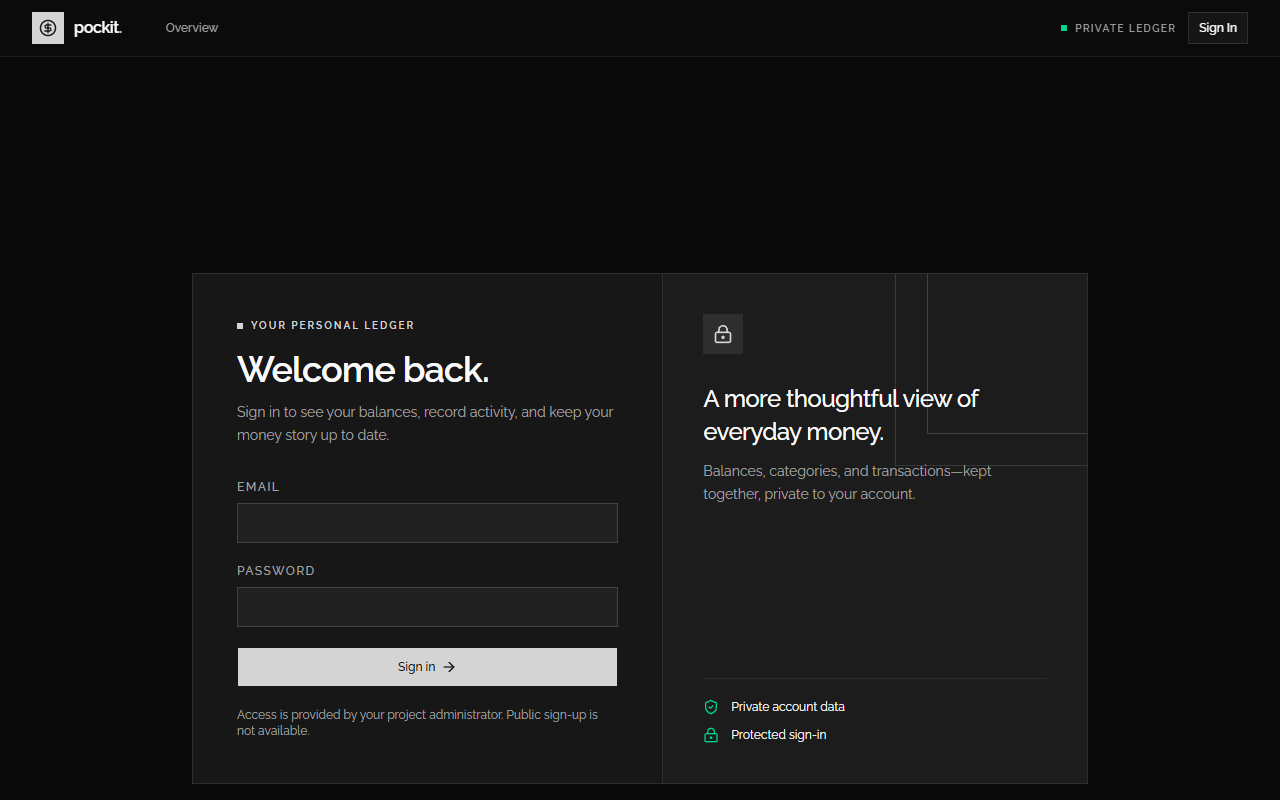
\includegraphics[width=0.98\linewidth,height=110mm,keepaspectratio]{evidence/f3-signed-out-login.png}\par\smallskip
    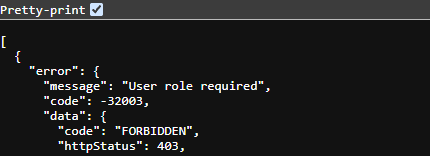
\includegraphics[width=0.98\linewidth,height=60mm,keepaspectratio]{evidence/f3-admin-finance-forbidden.png}
  \end{center}
  Automated tests at \TestFileLink{apps/server/src/auth.test.ts} cover valid/invalid credentials, current identity, and logout. Finance access tests at \TestFileLink{packages/api/src/routers/finance.test.ts} reject cross-User and Administrator access.
\end{tcolorbox}
\clearpage

\subsection{Recorded build, test, and migration results}
The full suite was rerun on 9 November 2026 with Bun 1.4.4 against an isolated PostgreSQL 17 database. The tested commit is \TestCommitLink{}; its Git tree matches the released tag \ReleaseTagLink{}. The temporary database used port 55441 and was removed after the run. The screenshots came from a separate student-run browser walkthrough; the assistant did not start or stop a development server.

\begin{longtable}{@{}p{0.25\textwidth}p{0.40\textwidth}p{0.25\textwidth}@{}}
\toprule
\textbf{Check} & \textbf{Command / conditions recorded} & \textbf{Result} \\\midrule
Full workspace tests & \texttt{DATABASE\_URL=<isolated> mise exec -- bun run test}; Bun 1.4.4, PostgreSQL 17, four migrations. & PASS: 51 total; 51 pass, 0 fail, no skipped tests reported. API 21, server 14, web 14, DB 2. \\
Workspace type-check/build tasks & \texttt{VITE\_SERVER\_URL=http://localhost:3000 DATABASE\_URL=<disposable> bun run check-types}. & PASS: all 6 Turbo tasks; web production client/SSR/Nitro build completed. Existing Rolldown module-directive warnings were non-fatal. \\
Direct API regression & \texttt{cd packages/api; bun test --timeout 5000}. & PASS: 21 tests in one Bun process on Bun 1.4.4; reported duration 2.80 seconds. \\
Session-race regression & Targeted \TestFileLink{apps/server/src/auth.test.ts} against disposable PostgreSQL; full command in \PartLink{E}{Part E}. & PASS: 10 tests, 43 assertions. Without the guard, the test first found one remaining session instead of zero. \\
Versioned migrations & \texttt{DATABASE\_URL=<isolated> mise exec -- bun run db:migrate:deploy}. & PASS: all four checked-in migrations applied to the disposable test DB. \\
Targeted style/diff checks & Targeted Biome on changed source/config files; \texttt{git diff --check}. & PASS on recorded targeted checks. A prior project-setup baseline \texttt{bun run check} failed with pre-existing diagnostics and is not reported as a pass. \\
\bottomrule
\end{longtable}

\noindent Full command output is retained in \path{evidence/workspace-test-output.txt}. The excerpt shows the package summaries; Bun reported no skipped tests.
\begin{lstlisting}
server:test:  14 pass
server:test:  0 fail
server:test: Ran 14 tests across 4 files. [7.03s]
@Pockit/api:test:  21 pass
@Pockit/api:test:  0 fail
@Pockit/api:test: Ran 21 tests across 4 files. [1398.00ms]
web:test:  14 pass
web:test:  0 fail
web:test: Ran 14 tests across 5 files. [37.32s]
@Pockit/db:test:  2 pass
@Pockit/db:test:  0 fail
@Pockit/db:test: Ran 2 tests across 1 file. [238.00ms]
\end{lstlisting}

\subsection{Acceptance-criteria to actual-test crosswalk}
The table maps all 43 acceptance criteria to planned STS IDs, actual test evidence, and results. The register links each evidence key to a test file or project record. \PartLink{E}{Part E} contains test conditions and limitations.
\subparagraph*{Actual test evidence register}
\noindent\small Evidence keys resolve to source files and representative test cases or process artifacts.\\[-2pt]
\setlength{\tabcolsep}{2pt}
\renewcommand{\arraystretch}{1.02}
\begin{longtable}{@{}>{\raggedright\arraybackslash}p{0.07\textwidth}>{\raggedright\arraybackslash}p{0.86\textwidth}@{}}
\toprule
\textbf{Ref.} & \textbf{Actual test or process evidence} \\
\midrule
\endfirsthead
\toprule
\textbf{Ref.} & \textbf{Actual test or process evidence} \\
\midrule
\endhead
\midrule\multicolumn{2}{r}{\footnotesize Continued on next page} \\
\endfoot
\bottomrule
\endlastfoot
\textbf{E01} & \href{https://github.com/ovenmakemeheat/Pockit/blob/28a0093535eb36d93f3d05dc2527d30cd4ccb32a/apps/server/src/auth.test.ts}{\path{apps/server/src/auth.test.ts}}: HTTP authentication and session tests \\
\textbf{E02} & \href{https://github.com/ovenmakemeheat/Pockit/blob/28a0093535eb36d93f3d05dc2527d30cd4ccb32a/packages/api/src/routers/finance.test.ts}{\path{packages/api/src/routers/finance.test.ts}}: finance authorization and ledger tests \\
\textbf{E03} & \href{https://github.com/ovenmakemeheat/Pockit/blob/28a0093535eb36d93f3d05dc2527d30cd4ccb32a/packages/api/src/routers/admin.test.ts}{\path{packages/api/src/routers/admin.test.ts}}: Administrator access-management tests \\
\textbf{E04} & \href{https://github.com/ovenmakemeheat/Pockit/blob/28a0093535eb36d93f3d05dc2527d30cd4ccb32a/apps/server/src/seed-data.test.ts}{\path{apps/server/src/seed-data.test.ts}}: synthetic seed tests \\
\textbf{E05} & \href{https://github.com/ovenmakemeheat/Pockit/blob/28a0093535eb36d93f3d05dc2527d30cd4ccb32a/packages/api/src/finance/value.test.ts}{\path{packages/api/src/finance/value.test.ts}}: exact-money and date validation tests \\
\textbf{E06} & \href{https://github.com/ovenmakemeheat/Pockit/blob/28a0093535eb36d93f3d05dc2527d30cd4ccb32a/packages/api/src/routers/finance.test.ts}{\path{packages/api/src/routers/finance.test.ts}}: database-backed finance journey and rejection tests \\
\textbf{E07} & \href{https://github.com/ovenmakemeheat/Pockit/blob/28a0093535eb36d93f3d05dc2527d30cd4ccb32a/apps/server/src/finance-persistence.test.ts}{\path{apps/server/src/finance-persistence.test.ts}}: fresh-client persistence test \\
\textbf{E08} & \href{https://github.com/ovenmakemeheat/Pockit/blob/28a0093535eb36d93f3d05dc2527d30cd4ccb32a/apps/web/src/components/finance-dashboard.test.tsx}{\path{apps/web/src/components/finance-dashboard.test.tsx}}: finance UI component tests \\
\textbf{E09} & \href{https://github.com/ovenmakemeheat/Pockit/blob/28a0093535eb36d93f3d05dc2527d30cd4ccb32a/apps/web/src/components/sign-in-form.test.tsx}{\path{apps/web/src/components/sign-in-form.test.tsx}}: login UI tests \\
\textbf{E10} & \href{https://github.com/ovenmakemeheat/Pockit/blob/28a0093535eb36d93f3d05dc2527d30cd4ccb32a/apps/web/src/components/admin-user-management.test.tsx}{\path{apps/web/src/components/admin-user-management.test.tsx}}: Administrator UI test \\
\textbf{E11} & \href{https://github.com/ovenmakemeheat/Pockit/blob/28a0093535eb36d93f3d05dc2527d30cd4ccb32a/apps/web/src/utils/user-scoped-query-key.test.ts}{\path{apps/web/src/utils/user-scoped-query-key.test.ts}}: cross-User cache isolation test \\
\textbf{E12} & \href{https://github.com/ovenmakemeheat/Pockit/blob/feature/working-sprint1/docs/testing/sprint1-software-test-specification.md}{\path{docs/testing/sprint1-software-test-specification.md}}: full AC/test mapping and execution record \\
\textbf{E13} & \href{https://github.com/ovenmakemeheat/Pockit/issues/5}{Issue \#5}; \href{https://github.com/ovenmakemeheat/Pockit/issues/7}{Issue \#7}; \href{https://github.com/ovenmakemeheat/Pockit/issues/8}{Issue \#8}; \href{https://github.com/ovenmakemeheat/Pockit/pull/20}{PR \#20}; \href{https://github.com/ovenmakemeheat/Pockit/pull/22}{PR \#22}; \href{https://github.com/ovenmakemeheat/Pockit/pull/27}{PR \#27}: review, integration, release, and board links \\
\end{longtable}
\medskip
\noindent\small All 43 stable criteria are retained. Evidence keys resolve above; outcomes follow the recorded STS result.\par
\setlength{\tabcolsep}{2pt}
\renewcommand{\arraystretch}{1.04}
\begin{longtable}{@{}>{\raggedright\arraybackslash}p{0.085\textwidth}>{\raggedright\arraybackslash}p{0.46\textwidth}>{\raggedright\arraybackslash}p{0.22\textwidth}>{\raggedright\arraybackslash}p{0.12\textwidth}@{}}
\toprule
\textbf{AC} & \textbf{Planned STS IDs} & \textbf{Actual evidence ref.} & \textbf{Result} \\
\midrule
\endfirsthead
\toprule
\textbf{AC} & \textbf{Planned STS IDs} & \textbf{Actual evidence ref.} & \textbf{Result} \\
\midrule
\endhead
\midrule\multicolumn{4}{r}{\footnotesize Continued on next page} \\
\endfoot
\bottomrule
\endlastfoot
\mbox{F1-AC-01} & \mbox{STS-AUTH-01}, \mbox{STS-AUTH-02}, \mbox{STS-UI-01} & E01, E09 & PASS \\
\mbox{F1-AC-02} & \mbox{STS-AUTH-03}, \mbox{STS-UI-01}, \mbox{STS-INT-03} & E01, E09, E02, E04 & PARTIAL \\
\mbox{F1-AC-03} & \mbox{STS-AUTH-01}, \mbox{STS-AUTH-05}, \mbox{STS-AUTH-10} & E01 & PASS \\
\mbox{F1-AC-04} & \mbox{STS-AUTH-04} & E01 & PASS \\
\mbox{F1-AC-05} & \mbox{STS-AUTH-06}, \mbox{STS-AUTH-09} & E01 & PASS \\
\mbox{F1-AC-06} & \mbox{STS-AUTH-07}, \mbox{STS-AUTH-08}, \mbox{STS-AUTH-11} & E01 & PASS \\
\mbox{F2-AC-01} & \mbox{STS-AUTHZ-02} & E02 & PASS \\
\mbox{F2-AC-02} & \mbox{STS-AUTHZ-03}, \mbox{STS-AUTHZ-04}, \mbox{STS-AUTHZ-05}, \mbox{STS-INT-03} & E02, E01, E04 & PASS \\
\mbox{F2-AC-03} & \mbox{STS-AUTHZ-07}, \mbox{STS-UI-03} & E03, E10 & PARTIAL \\
\mbox{F2-AC-04} & \mbox{STS-AUTHZ-01}, \mbox{STS-AUTHZ-06} & E02, E03 & PASS \\
\mbox{F2-AC-05} & \mbox{STS-AUTHZ-08}, \mbox{STS-UI-03} & E02, E03, E10 & PARTIAL \\
\mbox{F2-AC-06} & \mbox{STS-AUTH-07}, \mbox{STS-AUTH-08}, \mbox{STS-AUTHZ-09}, \mbox{STS-AUTH-11} & E01, E03 & PASS \\
\mbox{F3-AC-01} & \mbox{STS-SEED-01} & E04 & PASS \\
\mbox{F3-AC-02} & \mbox{STS-SEED-02} & E04 & PASS \\
\mbox{F3-AC-03} & \mbox{STS-SEED-03} & E04 & PASS \\
\mbox{F3-AC-04} & \mbox{STS-SEED-04}, \mbox{STS-INT-03} & E04, E01, E02 & PASS \\
\mbox{F3-AC-05} & \mbox{STS-AUTHZ-07}, \mbox{STS-AUTHZ-08} & E03, E02 & PASS \\
\mbox{F4-AC-01} & \mbox{STS-OPEN-01} & E06 & PASS \\
\mbox{F4-AC-02} & \mbox{STS-OPEN-02} & E06 & PASS \\
\mbox{F4-AC-03} & \mbox{STS-OPEN-03} & E02, E06 & PASS \\
\mbox{F4-AC-04} & \mbox{STS-OPEN-04} & E05 & PASS \\
\mbox{F4-AC-05} & \mbox{STS-OPEN-05}, \mbox{STS-OPEN-06}, \mbox{STS-INT-02} & E05, E06 & PASS \\
\mbox{F5-AC-01} & \mbox{STS-RECEIVE-01}, \mbox{STS-RECEIVE-05} & E06, E05 & PASS \\
\mbox{F5-AC-02} & \mbox{STS-RECEIVE-01}, \mbox{STS-RECEIVE-06} & E06, E07 & PASS \\
\mbox{F5-AC-03} & \mbox{STS-RECEIVE-02}, \mbox{STS-RECEIVE-03}, \mbox{STS-RECEIVE-05} & E06, E05 & PASS \\
\mbox{F5-AC-04} & \mbox{STS-RECEIVE-04}, \mbox{STS-AUTHZ-05} & E02, E06 & PASS \\
\mbox{F5-AC-05} & \mbox{STS-RECEIVE-01}, \mbox{STS-VIEW-02} & E06, E08 & PASS \\
\mbox{F6-AC-01} & \mbox{STS-CARD-07}, \mbox{STS-CARD-01}, \mbox{STS-INT-02} & E06, E08, E05 & PASS \\
\mbox{F6-AC-02} & \mbox{STS-CARD-03} & E06 & PASS \\
\mbox{F6-AC-03} & \mbox{STS-CARD-01}, \mbox{STS-CARD-03}, \mbox{STS-CARD-05}, \mbox{STS-CARD-07} & E06, E08, E07 & PASS \\
\mbox{F6-AC-04} & \mbox{STS-CARD-02}, \mbox{STS-CARD-04}, \mbox{STS-CARD-06} & E06, E02 & PASS \\
\mbox{F6-AC-05} & \mbox{STS-CARD-01}, \mbox{STS-CARD-03}, \mbox{STS-CARD-05}, \mbox{STS-VIEW-02} & E06, E08, E07 & PASS \\
\mbox{F7-AC-01} & \mbox{STS-CARD-05}, \mbox{STS-VIEW-01}, \mbox{STS-UI-02} & E06, E07, E08 & PASS \\
\mbox{F7-AC-02} & \mbox{STS-CARD-05}, \mbox{STS-VIEW-02}, \mbox{STS-VIEW-03}, \mbox{STS-UI-02} & E06, E07, E08 & PASS \\
\mbox{F7-AC-03} & \mbox{STS-OPEN-04}, \mbox{STS-VIEW-03}, \mbox{STS-VIEW-04}, \mbox{STS-UI-02}, \mbox{STS-UI-04} & E05, E06, E08, E02, E11 & PASS \\
\mbox{F7-AC-04} & \mbox{STS-RECEIVE-06}, \mbox{STS-VIEW-05}, \mbox{STS-UI-02} & E07, E08 & PASS \\
\mbox{F7-AC-05} & \mbox{STS-OPEN-04}, \mbox{STS-OPEN-05}, \mbox{STS-VIEW-02}, \mbox{STS-VIEW-06}, \mbox{STS-UI-02} & E05, E06, E08 & PASS \\
\mbox{F8-AC-01} & \mbox{STS-OPEN-05}, \mbox{STS-RECEIVE-01}, \mbox{STS-CARD-01}, \mbox{STS-CARD-03}, \mbox{STS-CARD-05}, \mbox{STS-CARD-07}, \mbox{STS-VIEW-01}, \mbox{STS-INT-02} & E05, E06, E08, E07 & PASS \\
\mbox{F8-AC-02} & \mbox{STS-AUTHZ-04}, \mbox{STS-AUTHZ-05}, \mbox{STS-OPEN-03}, \mbox{STS-RECEIVE-02}, \mbox{STS-RECEIVE-03}, \mbox{STS-CARD-02}, \mbox{STS-CARD-04}, \mbox{STS-INT-01} & E02, E06 & PASS \\
\mbox{F8-AC-03} & \mbox{STS-AUTHZ-01}, \mbox{STS-AUTHZ-02}, \mbox{STS-AUTHZ-03}, \mbox{STS-AUTHZ-04}, \mbox{STS-AUTHZ-05}, \mbox{STS-AUTHZ-06}, \mbox{STS-AUTHZ-07}, \mbox{STS-AUTHZ-08}, \mbox{STS-AUTHZ-09}, \mbox{STS-AUTH-11}, \mbox{STS-RECEIVE-04}, \mbox{STS-CARD-02}, \mbox{STS-CARD-04}, \mbox{STS-VIEW-04}, \mbox{STS-UI-03}, \mbox{STS-UI-04} & E02, E03, E01, E06, E10, E11 & PASS \\
\mbox{F8-AC-04} & \mbox{STS-AUTH-06}, \mbox{STS-SEED-04}, \mbox{STS-INT-03} & E01, E04, E02 & PASS \\
\mbox{F8-AC-05} & This AC→STS table plus actual test/\allowbreak{}result/\allowbreak{}commit record in Issue \#8 & E12 & PARTIAL \\
\mbox{F8-AC-06} & Reviewed PR/\allowbreak{}issue history and project-board/\allowbreak{}checklist state before Issue \#8 implementation & E13 & PARTIAL \\
\end{longtable}
\normalsize
\setlength{\tabcolsep}{6pt}
\renewcommand{\arraystretch}{1.15}


\subsection{Selected excerpts of actual automated tests}
\textbf{Business-rule test.} This test rejects an allocation mismatch, then checks that the database state did not change. The source is \TestFileLink{packages/api/src/routers/finance.test.ts}, in the test named \emph{rejects invalid transaction inputs without changing ledger state}. The test passed in the API and root suites.
\begin{lstlisting}
for (const input of invalidWrites) {
  await expectRejectedWithCode(
    api.finance.transactions.create(input as never),
    "BAD_REQUEST",
  );
}

const [transactionsAfter, allocationsAfter, summaryAfter, bankAfter, cardAfter] =
  await Promise.all([
    db.financialTransaction.count({ where: { ownerId: ids.userA } }),
    db.allocationLine.count({ where: { ownerId: ids.userA } }),
    api.finance.summary.get(),
    api.finance.accounts.get({ accountId: accounts.bank }),
    api.finance.accounts.get({ accountId: accounts.card }),
  ]);
expect(transactionsAfter).toBe(transactionsBefore);
expect(allocationsAfter).toBe(allocationsBefore);
expect(summaryAfter).toEqual(summaryBefore);
expect(bankAfter.balance).toBe(bankBefore.balance);
expect(cardAfter.balance).toBe(cardBefore.balance);
\end{lstlisting}

\textbf{Ownership test.} This API test rejects a foreign User's Account lookup and an allocation to that User's Account. It confirms that neither User's transaction count changes. The source is \TestFileLink{packages/api/src/routers/finance.test.ts}, in the test named \emph{does not disclose another User account and rejects cross-owner writes}.
\begin{lstlisting}
await expectRejectedWithCode(
  api.finance.accounts.get({ accountId: accounts.userBBank }),
  "NOT_FOUND",
);
await expectRejectedWithCode(
  api.finance.transactions.create({
    form: "RECEIVE_MONEY",
    sourceAccountId: accounts.bank,
    totalAmount: "1.00",
    transactionDate: "2026-11-04",
    allocations: [
      { kind: "INCOME", accountId: accounts.userBBank, amount: "1.00" },
    ],
  }),
  "BAD_REQUEST",
);
expect(await db.financialTransaction.count({ where: { ownerId: ids.userA } }))
  .toBe(countBeforeA);
expect(await db.financialTransaction.count({ where: { ownerId: ids.userB } }))
  .toBe(countBeforeB);
\end{lstlisting}

\subsection{Selected issue and PR evidence}
The short history is requirements/design, reviewed Sprint 1 contracts, implementation, then a reviewed release to \texttt{main}. The linked Issues and PRs hold the full discussion and change history.
\begin{longtable}{@{}p{0.20\textwidth}p{0.32\textwidth}p{0.42\textwidth}@{}}
\toprule
\textbf{Issue / PR} & \textbf{Branch and authorship} & \textbf{Substantive review / result} \\\midrule
\IssueLink{5} / \PRLink{20} & \BranchLink{docs/system-level-sds}; \texttt{staging-1} to \texttt{staging-1}. Author: \UserLink{ovenmakemeheat}{Guntee}. & \UserLink{MadMax168}{Polwarit} reviewed architecture, data model, privacy, and deployment. Requested OQ-02's excess-precision/no-rounding policy remain proposed until confirmation. Merged. \\
\IssueLink{7} / \PRLink{22} & \ContractBranchLink{}; \texttt{staging-1} to \texttt{staging-1}. Author: \UserLink{ovenmakemeheat}{Guntee}. & \UserLink{MadMax168}{Polwarit} reviewed FEAT-01–FEAT-08 and the STS. Requested valid one-line purchases remain allowed while the demo still splits across two categories. Merged. \\
\IssueLink{8} / \PRLink{27} & Sprint 1 release from \texttt{staging-1} to \texttt{main}. & Reviewed by \UserLink{MadMax168}{Polwarit}; released at \ReleaseCommitLink{} and tagged \ReleaseTagLink{}. Implementation and regression PRs are linked from \IssueLink{8}. \\
\bottomrule
\end{longtable}
\noindent Board status: \IssueLink{5} and \IssueLink{7} are Done; \IssueLink{8} remains Started while this report is finalized. See the \BoardLink{}.

\subsection{Contribution and AI-use record}
\begin{longtable}{@{}L{0.34\textwidth}L{0.63\textwidth}@{}}
\toprule
\textbf{Student} & \textbf{Repository-visible contribution} \\\midrule
\UserLink{ovenmakemeheat}{Guntee Doungmanee}, 67070501003 & Requirements, design, implementation, tests, and report authorship. See \IssueLink{3}–\IssueLink{8} and \PRLink{18}–\PRLink{27}. \\
\UserLink{MadMax168}{Polwarit Watthanahemmarat}, 67070501067 & Requirements/design and test review, implementation reviews, release review, and setup confirmation. See the reviews linked above. \\
\bottomrule
\end{longtable}
\noindent\textbf{AI-use record.} Guntee used Pi's coding assistant, including bounded review agents, for requirements, implementation, tests, debugging, review, and report preparation. Prompts below are representative paraphrases, not a transcript. Guntee reviewed generated changes and test results; Polwarit provided independent reviews recorded in the linked PRs. The students made project decisions. AI output was not treated as test evidence.\par\medskip
\footnotesize
\setlength{\tabcolsep}{3pt}
\renewcommand{\arraystretch}{1.08}
\begin{longtable}{@{}L{0.14\textwidth}L{0.18\textwidth}L{0.40\textwidth}L{0.22\textwidth}@{}}
\toprule
\textbf{Use case} & \textbf{Technique} & \textbf{Representative prompt (paraphrased)} & \textbf{Human check} \\\midrule
Requirements & Source-grounded extraction and synthesis. & ``Use Theme 7 in the assignment to draft the SRS, traceability, and sprint plan. Keep unconfirmed decisions open.'' & Compared with the assignment; reviewed through \IssueLink{3}--\IssueLink{7} and \PRLink{18}--\PRLink{22}. \\
Code/tests & Code and test drafting, then targeted revision. & ``Implement Issue \#8's finance journey. Test persistence, invalid transactions, cross-User access, and Administrator denial.'' & Reviewed diffs and ran recorded tests; gaps remain listed in Part F and the STS. \\
Debug/review & Error-driven diagnosis and bounded specialist review. & ``Find why the finance test stalls; verify the cause and whether the fix completes normally.'' \newline ``Review the PR for authorization and session-race defects; report actionable findings.'' & Reproduced and checked test behavior; human teammate reviews and dispositions are linked in \PRLink{23}--\PRLink{27}. \\
Report & Scripted extraction, ID checks, LaTeX generation, and PDF inspection. & ``Condense Parts A--F into tables; preserve every stable ID, add links, and render the Mermaid diagrams.'' & Ran generator tests and LaTeX build; checked IDs, links, diagrams, screenshots, and page layout. \\
\bottomrule
\end{longtable}
\normalsize
\setlength{\tabcolsep}{6pt}
\renewcommand{\arraystretch}{1.15}

\subsection{Limitations}
\begin{itemize}
  \item Browser-level route/role journeys and structured log-redaction assertions were not verified. API and component tests provide the recorded evidence.
  \item The session-race regression has a recorded pre-fix failure and post-fix pass. Pre-implementation failure output for the original financial rules was not retained, so this report does not claim test-first evidence for those changes.
  \item The earlier full \texttt{bun run check} reported existing baseline diagnostics; only the listed targeted Biome checks passed.
  \item OQ-01, OQ-04, OQ-06, and OQ-07 remain open as recorded in \PartLink{A}{Part A}. Docker/GCP deployment is planned for Lab 5; no cloud deployment is claimed.
  \item Both students should confirm the contribution summary before submission.
\end{itemize}

\label{part:F:end}
\end{document}
